\documentclass[
    % -- opções da classe memoir --
    12pt,               % tamanho da fonte
    openright,          % capítulos começam em pág ímpar (insere página vazia caso preciso)
    %twoside,            % para impressão em verso e anverso. Oposto a oneside
    oneside,
    a4paper,            
    english,            % idioma adicional para hifenização
    brazil              % o último idioma é o principal do documento
    ]{abntex2}

% ---
% Pacotes básicos 
% ---
\usepackage{lmodern}            % Usa a fonte Latin Modern          
\usepackage[T1]{fontenc}        % Selecao de codigos de fonte.
\usepackage[utf8]{inputenc}     % Codificacao do documento (conversão automática dos acentos)
\usepackage{lastpage}           % Usado pela Ficha catalográfica
\usepackage{indentfirst}        % Indenta o primeiro parágrafo de cada seção.
\usepackage{color}              % Controle das cores
\usepackage{graphicx}           % Inclusão de gráficos
\usepackage{microtype}          % para melhorias de justificação
\usepackage{amssymb,amsmath}
\usepackage{color, colortbl}
\usepackage{tikz}
\usepackage{schemabloc}
\usepackage{subfig}
\usepackage{listings}
\usepackage{pgf-umlsd}
\usetikzlibrary{shapes,arrows}

\usetikzlibrary{circuits}
% ---

\usetikzlibrary{plotmarks}
        
% ---
% Pacotes adicionais, usados apenas no âmbito do Modelo Canônico do abnteX2
% ---
\usepackage{lipsum}             % para geração de dummy text
% ---

% ---
% Pacotes de citações
% ---
\usepackage[brazilian,hyperpageref]{backref}     % Paginas com as citações na bibl
%\usepackage[alf]{abntex2cite}   % Citações padrão ABNT

% --- 
% CONFIGURAÇÕES DE PACOTES
% --- 

% ---
% Configurações do pacote backref
% Usado sem a opção hyperpageref de backref
\renewcommand{\backrefpagesname}{Citado na(s) página(s):~}
% Texto padrão antes do número das páginas
\renewcommand{\backref}{}
% Define os textos da citação
\renewcommand*{\backrefalt}[4]{
    \ifcase #1 %
        Nenhuma citação no texto.%
    \or
        Citado na página #2.%
    \else
        Citado #1 vezes nas páginas #2.%
    \fi}%
% ---

% ---
% Informações de dados para CAPA e FOLHA DE ROSTO
% ---
\titulo{Estudo e desenvolvimento de sistema de detecção de som para identificação de focos de poluição sonora na cidade do Recife}

\autor{Thiago Oliveira Ribeiro}

\local{Recife - PE, Brasil}

\data{novembro de 2015}

\orientador{Prof. Sérgio Campello Oliveira}

\coorientador{}

\instituicao{%
  Engenharia de Computação
  \par
  Escola Politécnica de Pernambuco
  \par
  Universidade de Pernambuco}
\tipotrabalho{Trabalho de Conclusão de Curso}
% O preambulo deve conter o tipo do trabalho, o objetivo, 
% o nome da instituição e a área de concentração 
\preambulo{Monografia apresentada como requisito parcial para obtenção do diploma de Bacharel em Engenharia de Computação pela Escola Politécnica de Pernambuco – Universidade de Pernambuco.}
% ---


% ---
% Configurações de aparência do PDF final

% alterando o aspecto da cor azul
%\definecolor{blue}{RGB}{41,5,195}
\definecolor{blue}{RGB}{0, 0, 0}

% informações do PDF
\makeatletter
\hypersetup{
        %pagebackref=true,
        pdftitle={\@title}, 
        pdfauthor={\@author},
        pdfsubject={\imprimirpreambulo},
        pdfcreator={LaTeX with abnTeX2},
        pdfkeywords={abnt}{latex}{abntex}{abntex2}{trabalho acadêmico}, 
        colorlinks=true,            % false: boxed links; true: colored links
        linkcolor=blue,             % color of internal links
        citecolor=blue,             % color of links to bibliography
        filecolor=magenta,              % color of file links
        urlcolor=blue,
        bookmarksdepth=4
}
\makeatother
% --- 

% --- 
% Espaçamentos entre linhas e parágrafos 
% --- 

% O tamanho do parágrafo é dado por:
\setlength{\parindent}{1.3cm}

% Controle do espaçamento entre um parágrafo e outro:
\setlength{\parskip}{0.2cm}  % tente também \onelineskip

%\OnehalfSpacing

% ---
% compila o indice
% ---
\makeindex
% ---

% ----
% Início do documento
% ----
\begin{document}
\lstset{language=C, linewidth=6cm} 

% Seleciona o idioma do documento (conforme pacotes do babel)
%\selectlanguage{english}
\selectlanguage{brazil}

% Retira espaço extra obsoleto entre as frases.
\frenchspacing 

% ----------------------------------------------------------
% ELEMENTOS PRÉ-TEXTUAIS
% ----------------------------------------------------------
% \pretextual

  \thispagestyle{empty}

  \begin{figure}[!htp]
    {
\includegraphics[scale=0.2, width=2.4cm]{../imagens/poli.png}}\hfill%
    {
\includegraphics[scale=0.3, width=3.7cm]{../imagens/ecomp.png}}%
  \end{figure}

  \begin{center}
      \vspace*{3.5cm}
      \Large\textbf{{Estudo e desenvolvimento de sistema de detecção de som para identificação de focos de poluição sonora na cidade do Recife}}
      \vskip 2cm
      \Large\textsf{Trabalho de Conclusão de Curso}\\[0.5cm]      
      \Large\textsf{Engenharia de Computação}
      \vskip 4.7cm
  \end{center}

  \begin{center}
    \large\textsc{{Thiago Oliveira Ribeiro}}\\
    \large{Orientador: Prof. Sérgio Campello Oliveira}
  \end{center}

  \begin{figure}[!htp]
    \centering
    
\includegraphics[scale=0.16]{../imagens/brasao.jpg}
  \end{figure}
% ---
% Capa
% ---
%\imprimircapa
% ---

% ---
% Folha de rosto
% (o * indica que haverá a ficha bibliográfica)
% ---
\imprimirfolhaderosto*
% ---

\begin{fichacatalografica}
    \sffamily
    \vspace*{\fill}                 % Posição vertical
    \begin{center}                  % Minipage Centralizado
    \fbox{\begin{minipage}[c][8cm]{13.5cm}      % Largura
    \small
    \imprimirautor
    %Sobrenome, Nome do autor
    
    \hspace{0.5cm} \imprimirtitulo  / \imprimirautor. --
    \imprimirlocal, \imprimirdata-
    
    \hspace{0.5cm} \pageref{LastPage} p. %: il. (algumas color.) ; 30 cm.\\
    
    \hspace{0.5cm} \imprimirorientadorRotulo~\imprimirorientador\\
    
    \hspace{0.5cm}
    \parbox[t]{\textwidth}{\imprimirtipotrabalho~--~\imprimirinstituicao,
    \imprimirdata.}\\
    

    \hspace{0.5cm}
        1. Som.
        2. Ruído.
        2. Recife.
        3. Detecção.
        4. Monitoramento.
        5. Internet.
        I. Prof. Sérgio Campello Oliveira.
        II. Universidade de Pernambuco.
        III. Escola Politécnica.
        IV. Título
    \end{minipage}}
    \end{center}
\end{fichacatalografica}
% ---

% ---
% Dedicatória
% ---
\begin{dedicatoria}
   \vspace*{\fill}
   \centering
   \noindent
   \textit{ Este trabalho é dedicado à minha família.} \vspace*{\fill}
\end{dedicatoria}
% ---

% ---
% Agradecimentos
% ---
\begin{agradecimentos}
Em primeiro lugar gostaria de agradecer a Deus, o Autor e Mantenedor de todas as coisas, No qual baseio minha fé, por ter sido meu refúgio indispensável nos mais delicados momentos que se passaram desde o início da minha graduação até aqui. 

Em segundo, à minha família: meus pais Enoque e Luciana e minha irmã Sara, por sempre acreditarem em mim e também por todo o incentivo e suporte em todas as horas.

À minha namorada Mari, por toda paciência, carinho e amor demonstrados durante todo esse tempo que se passou desde o conceito deste projeto até sua execução final.

Em especial gostaria de agradecer aos que chamo de \textit{guerreiros}. Aqueles que comigo viraram noites estudando, dedicaram tudo de si e fizeram parte da minha vida durante todos esses anos. Da primeira derivada e do primeiro laço de repetição até aqui, vocês foram peça chave nessa minha conquista. São eles meus amigos de UNIVASF: Bruno Sampaio, Washington Lacerda, José Matias, Eldon Costa, Danilo Macário, Ivonaldo Faustino, Renato Gabriel e Raí Tamarindo. Aos amigos do pensionato Lar do Estudante Daniel Pinheiro e José Elias, os quais acompanharam de perto algumas das etapas que passei longe de casa para chegar até aqui. Também de lá, diretamente do sertão, vai o meu agradecimento especial a um professor que marcou parte da minha graduação com sua maestria e paixão visíveis pela Matemática e pela Computação, Edson Araújo. 

Aos meus grandes amigos dos tempos de \textit{Oklahoma Christian University}, que fizeram do meu tempo nos Estados Unidos, um dos melhores da minha vida: Gustavo Moreira, Laércio Vitorino e Allan Amorim. 

Aos grandes amigos que fiz e levarei para vida toda, os quais fizeram da minha experiência na POLI algo muito melhor do que eu imaginei: Hartur Brito, Gemerson Gerardo, Felipe Jorge, Felipe Morais, Helson Cruz, Jhonatan Santos e Ivaldo Camelo. 

Aos meus amigos de Nerval: Lucas Nunes, Rafael Soares e Gildson Luiz. 

A todos os professores dedicados e comprometidos com os quais que tive a oportunidade de aprender, em especial aos do Ensino Fundamental e Médio, que muitas vezes não são lembrados, mas que para mim foram também peças indispensáveis na minha decisão em me tornar um Engenheiro de Computação. 

Ao meu professor orientador Sérgio Campello, por ter me passado parte do seu conhecimento em Eletrônica, pela gentileza e acompanhamento durante as etapas deste trabalho, o meu muito obrigado.


\end{agradecimentos}
% ---

\begin{epigrafe}
    \vspace*{\fill}
    \begin{flushright}
        \textit{``Truth is ever to be found  \\
                  in simplicity, and not \\ in the multiplicity 
                  and \\ confusion of things.''\\
        \textbf{Isaac Newton}}
    \end{flushright}
\end{epigrafe}

% ---
% RESUMOS
% ---

% resumo em português
\setlength{\absparsep}{18pt} % ajusta o espaçamento dos parágrafos do resumo
\begin{resumo}
 % Segundo a %\citeonline[3.1-3.2]{NBR6028:2003}, o resumo deve ressaltar o
 % objetivo, o método, os resultados e as conclusões do documento. A ordem e a extensão
 % destes itens dependem do tipo de resumo (informativo ou indicativo) e do
 % tratamento que cada item recebe no documento original. O resumo deve ser
 % precedido da referência do documento, com exceção do resumo inserido no
 % próprio documento. (\ldots) As palavras-chave devem figurar logo abaixo do
 % resumo, antecedidas da expressão Palavras-chave:, separadas entre si por
 % ponto e finalizadas também por ponto.

Recentemente, o aumento da poluição sonora no mundo e principalmente em áreas urbanas, tem sido encarado como um dos maiores problemas da sociedade moderna. Não menos danosa à saúde humana que outros tipos de poluição, a poluição sonora tem sido reconhecida como uma das maiores pertubações que afetam a qualidade de vida nas grandes cidades. Neste sentido, diversos órgãos de estado tem movido ações para combater a emissão de ruídos por parte de estabelecimentos, residências e centros com grande concentração de pessoas. O processo de controle desses níveis de som funciona a partir do envio de fiscais munidos de Medidores de Nível de Pressão Sonora para identificar locais infratores que estejam emitindo ruídos acima do permitido para determinados horários do dia. Por tratar-se de um processo demorado e sem possibilidade de monitoramento constante, o \textit{hardware} desevenvolvido neste projeto trata-se de um medidor de baixo custo montado em uma placa de prototipação, e um \textit{software} (\textit{mobile}) monitorador capaz de verificar em tempo real os níveis emitidos por locais da cidade do Recife, de modo a mapear e controlar a poluição sonora remotamente. O sistema comportou-se de maneira esperada ao ser capaz de medir valores em decibéis e enviá-los a um servidor \textit{web}, onde tais dados são exibidos em um \textit{software} desenvolvido para sistemas operacionais iOS.

 \textbf{Palavras-chave}: Som. Detecção. Ruído. Recife. Monitoramento. Arduino. WiFi.
\end{resumo}

% resumo em inglês
\begin{resumo}[Abstract]
 \begin{otherlanguage*}{english}
   Recently, the increase in noise pollution in the world and especially in urban areas, has been seen as one of the biggest problems of modern society. No less harmful to human health than other types of pollution, noise pollution has been recognized as one of the largest disturbances affecting the quality of life in big cities. In this regard, several state agencies have moved actions to combat the emission of noise by schools, residences and centers with large concentrations of people. The control process of these sound levels operates from sending officers using Sound Pressure Level Meters to identify offenders locations that are emitting above the allowed noise for certain times of day. As this is a long process without the possibility of constant monitoring, the project proposed aims to develop a low-cost hardware meter, and a mobile software tracker to be able to check real-time output levels by certain locations of Recife, in order to map and control noise pollution. The whole system worked as expected by being able to measure values in decibels and send them to a web server, from where they could be read and displayed in software (mobile app) developed for the iOS operating system.

   \vspace{\onelineskip}
 
   \noindent 
   \textbf{Keywords}: Sound. Noise. Detector. Monitoring. Arduino. WiFi.
 \end{otherlanguage*}
\end{resumo}

% ---
% inserir lista de ilustrações
% ---
\pdfbookmark[0]{\listfigurename}{lof}
\listoffigures*
\cleardoublepage
% ---

% ---
% inserir lista de tabelas
% ---
\pdfbookmark[0]{\listtablename}{lot}
\listoftables*
\cleardoublepage
% ---

% ---
% inserir lista de abreviaturas e siglas
% ---
\begin{siglas}
  \item[MNPS] Medidor de Nível de Pressão Sonora
  \item[DDS] Detector de Som
  \item[HTTP] \textit{Hypertext Transfer Protocol}
  \item[SPL] \textit{Sound Pressure Level}
  \item [IDE] \textit{Integrated Development Environment}
  \item [API] \textit{Application Programming Interface}
  \item [TCP/IP] \textit{Transmission Control Protocol / Internet Protocol}
\end{siglas}
% ---

% ---
% inserir lista de símbolos
% ---
% \begin{simbolos}
%   \item[$ \Gamma $] Letra grega Gama
%   \item[$ \Lambda $] Lambda
%   \item[$ \zeta $] Letra grega minúscula zeta
%   \item[$ \in $] Pertence
% \end{simbolos}
% ---

% ---
% inserir o sumario
% ---
\pdfbookmark[0]{\contentsname}{toc}
\tableofcontents*
\cleardoublepage
% ---

% ----------------------------------------------------------
% ELEMENTOS TEXTUAIS
% ----------------------------------------------------------
\textual

% ----------------------------------------------------------
% Introdução (exemplo de capítulo sem numeração, mas presente no Sumário)
% ----------------------------------------------------------
\chapter{Introdução}\label{introducao}
%\addcontentsline{toc}{chapter}{Introdução}
% ----------------------------------------------------------

Este trabalho de conclusão de curso propõe-se ao estudo e desenvolvimento de um projeto de sistema computacional (de \textit{hardware} e \textit{software}), que seja capaz de medir e monitorar a intensidade de ruído em certos pontos da cidade do Recife.

O crescente número de queixas de barulho excessivo por parte da população, e os diversos danos à saúde adventos deste tipo de poluição, foram alguns dos fatores que desencadearam a escolha deste tema.

Este capítulo descreve a introdução da monografia, e está organizado em 3 seções. Na Seção \ref{motivacao} são descritas tanto a motivação para a execução deste trabalho, quanto a definição do problema. 

Posteriormente, nas Seções \ref{geral} e \ref{especificos} são apresentados os objetivos gerais e específicos, bem como a proposta de solução do projeto. Por fim, a Seção \ref{estrutura} detalha a organização da monografia.

\section{Motivação e Caracterização do Problema}\label{motivacao}

Atualmente, a humanidade tem experimentado um de seus maiores males concebidos por si própria: a poluição sonora. Especialmente em áreas urbanas, essa forma de poluição, não menos preocupante que outras como atmosférica ou ambiental, tem sido devidamente reconhecida como uma das maiores perturbações que afetam a qualidade de vida nas grandes cidades \cite{majid}. 

O conceito de ruído geralmente refere-se a sons não desejados que possam afetar negativamente a vida humana ou animal \cite{enda}. 

De fato, em um típico ambiente urbano, rodeado de construções, avenidas movimentadas, bares e restaurantes, a população vivendo nesses centros encontra-se inevitalmente exposta a uma variedade desses sons, que além de interferir no seu bem-estar cotidiano, pode vir a trazer graves consequências à saúde, sendo uma das mais preocupantes a Perda Auditiva Induzida por Ruído (PAIR) \cite{tizi}. 

Segundo guia da \textit{World Health Organization} (WHO), agência da Organização das Nações Unidas (ONU) incumbida de assuntos ligados à saúde pública internacional, já em 1999 estimava que mais de 120 milhões de pessoas ao redor do mundo sofriam de PAIR devido a poluição sonora nos centros urbanos \cite{thomas}. 

No Brasil, o problema já é considerado um grave caso de saúde pública, contribuindo no aumento de depressão e outras graves doenças \cite{andre}. 

Sendo assim, pensando na redução e combate ao barulho excessivo, a Prefeitura da Cidade do Recife (PCR) junto ao Ministério Público de Pernambuco, secretarias e órgãos do Governo do Estado, firmaram uma parceria formalizando a responsabilidade de cada uma das instituições na fiscalização de estabelecimentos de serviços, lojas e bares da capital pernambucana \cite{secretaria}. 

Também, a fim de alertar sobre os prejuízos do excesso de ruído, foi atribuída a PCR, dentre outras definições, a de realizar campanhas educativas sobre o tema em estabelecimentos e escolas municipais e privadas com o intuito de multiplicar a informação \cite{secretaria}. 

Portanto, este trabalho visa mapear e controlar os altos níveis de ruído encontrados nos principais pontos da cidade do Recife, a partir do desenvolvimento de um sistema que monitore o som do ambiente no qual estiver instalado, e exiba estes dados de maneira autônoma, para que os órgãos competentes instruam o local emissor a amenizar o barulho no mesmo momento em que for detectado o excesso, a partir da medição viabilizada pelo sistema.

\section{Objetivo Geral}\label{geral}

Este trabalho tem como objetivo principal o estudo e implementação de um sistema computacional a partir de um projeto de \textit{hardware}, capaz de medir a intensidade do barulho gerado em certos locais da cidade do Recife, e de uma aplicação em \textit{software} que viabilize o acesso dos dados em qualquer lugar, identificando assim os locais emissores dos mais altos níveis de ruído.

\section{Objetivos Específicos}\label{especificos}

A implementação do projeto também envolveu outros fins, os quais foram atingidos:

  \begin{itemize}
    \item Estudo sobre a natureza do som e sua medição;
    \item Proposta e desenvolvimento de um medidor de baixo custo em \textit{hardware};
    \item Desenvolvimento de aplicação em \textit{software} para visualizar informações obtidas pelo medidor;
    \item Realização de testes do sistema em certo local na cidade do Recife. 
  \end{itemize}

\section{Estrutura do Documento}\label{estrutura}

Este trabalho está dividido em 5 capítulos, incluindo este que conta com uma introdução a respeito do tema e objetivos do projeto. Em seguida o Capítulo \ref{teoria} traz um estudo a respeito das propriedades do som, meios de medí-lo, e demais conceitos necessários para a compreensão do sistema desenvolvido neste trabalho. 

Já no Capítulo \ref{projeto}, é descrito as etapas do processo que resultou no sistema proposto. O Capítulo \ref{resultados} apresenta os resultados obtidos e dados de testes efetuados com o sistema em funcionamento. 

Finalmente, o Capítulo \ref{conclusao} encerra o trabalho com uma discussão a respeito do que foi desenvolvido, e possíveis melhoramentos e novas ideias para o projeto.

\chapter{Fundamentação Teórica}\label{teoria}

Este capítulo busca apresentar alguns conceitos fundamentais a respeito do som e suas características, bem como explicitar meios de medir sua intensidade. 

Também é detalhada a teoria que fundamenta os componentes e ferramentas utilizadas tanto no projeto do medidor em \textit{hardware}, quanto do \textit{software} de monitoração dos dados.

% Nas Seção \ref{som-definicao} é descrita a definição de som e alguns fundamentos do mesmo. Na Seção \ref{caracteristicas} temos...

% ----------------------------------------------------------
% FUNDAMENTOS E CONCEITO DE SOM
% ----------------------------------------------------------

\section{Fundamentos e Conceito de Som}\label{som-definicao}

De todas as formas de ondas mecânicas encontradas na natureza, uma das mais importantes são as \textit{ondas sonoras}. É possível categorizar ondas com base no movimento das partículas no meio em que a onda se propaga \cite{halliday}. Os dois tipos mais notáveis desta categoria são:

\begin{itemize}
  \item \textbf{Ondas Transversais:} são aquelas em que a direção de vibração das partículas no meio, é \textit{perpendicular} à direção de propagação da onda.

  \begin{figure}[!htb]
    \caption{\label{fig_onda-transversal}Exemplo de onda transversal em uma corda.}
    \begin{center}
    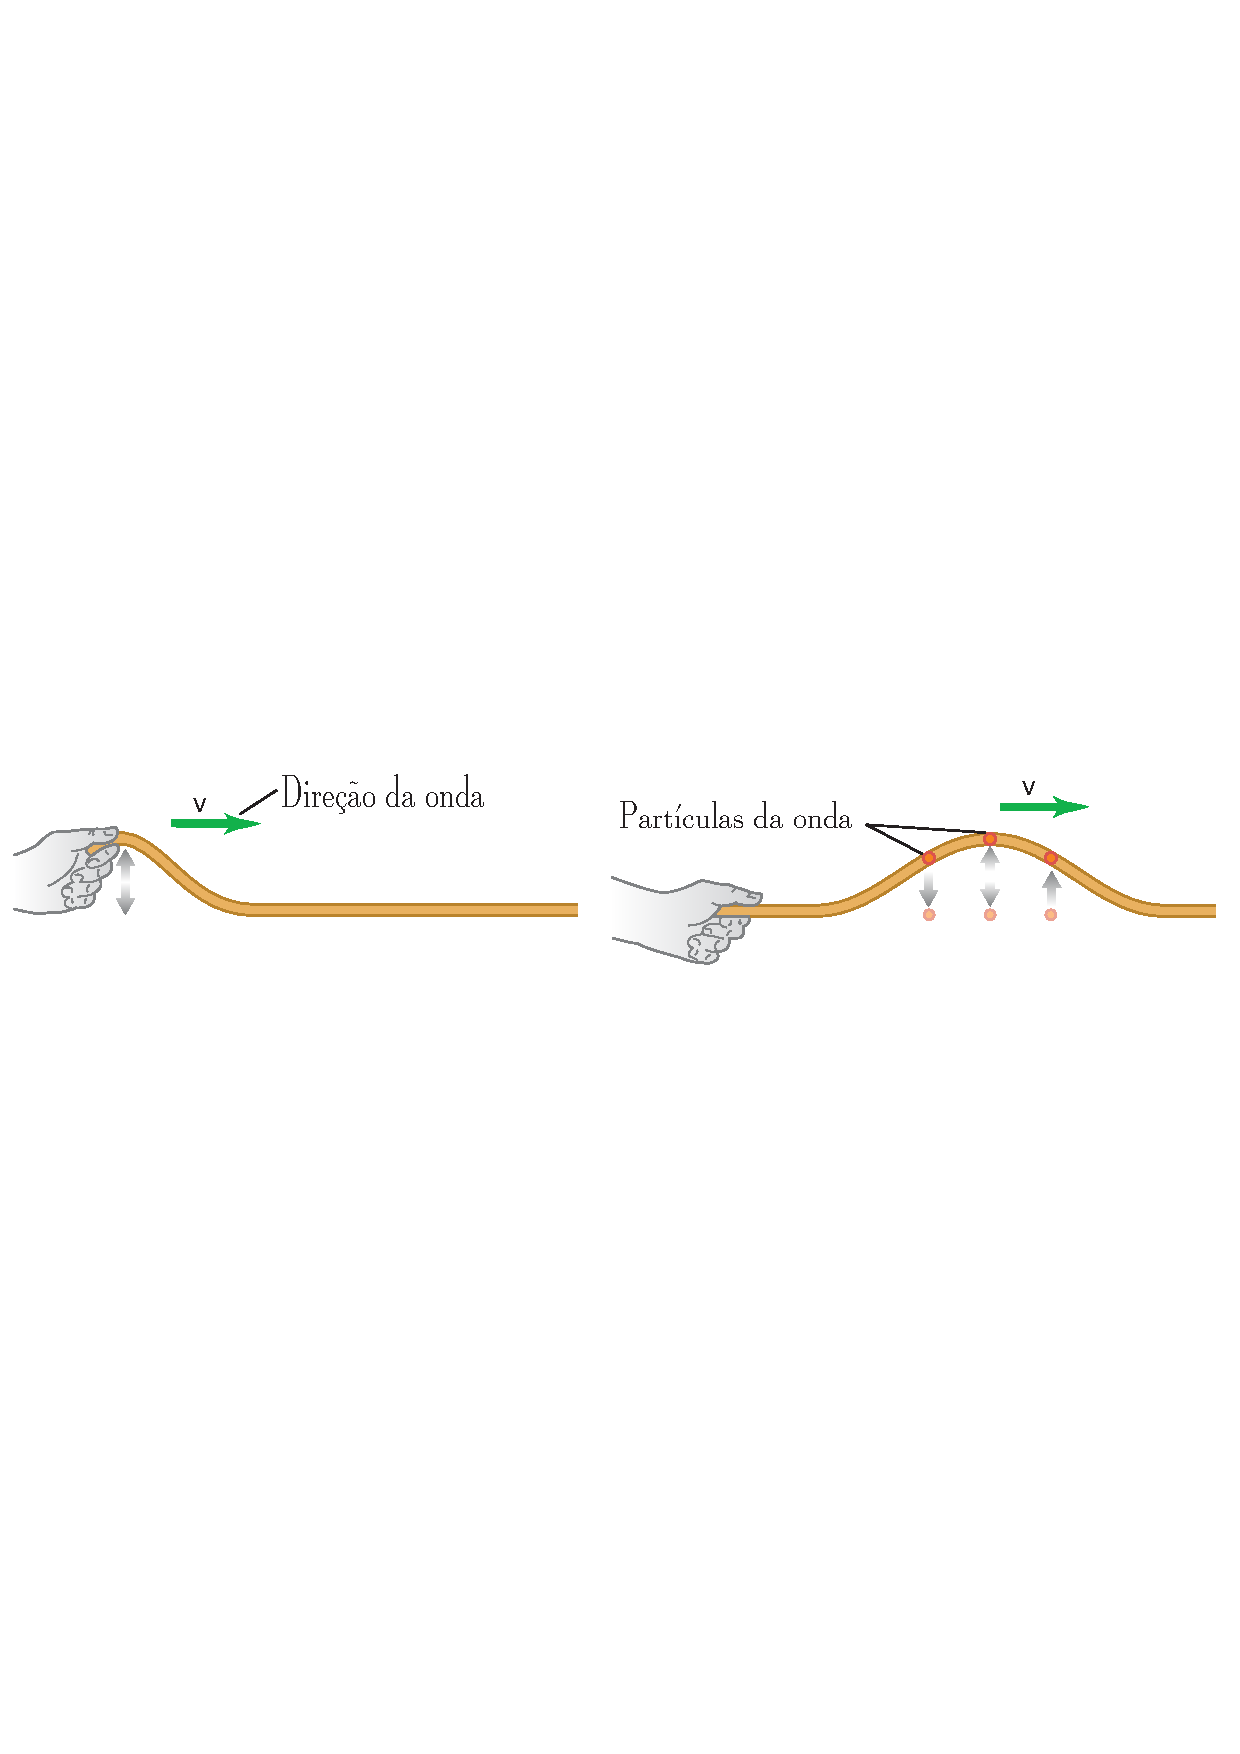
\includegraphics[scale=0.5]{images/img-1.pdf}
    \end{center}
    \legend{Fonte: extraído de \cite{young}.}
  \end{figure}

   \item \textbf{Ondas Longitudinais:} são aquelas em que a direção de vibração das partículas no meio, é \textit{paralela} à direção de propagação da onda.

  \begin{figure}[!htb]
    \caption{\label{fig_onda-longitudinal}Exemplo de onda longitudinal em um fluido.}
    \begin{center}
    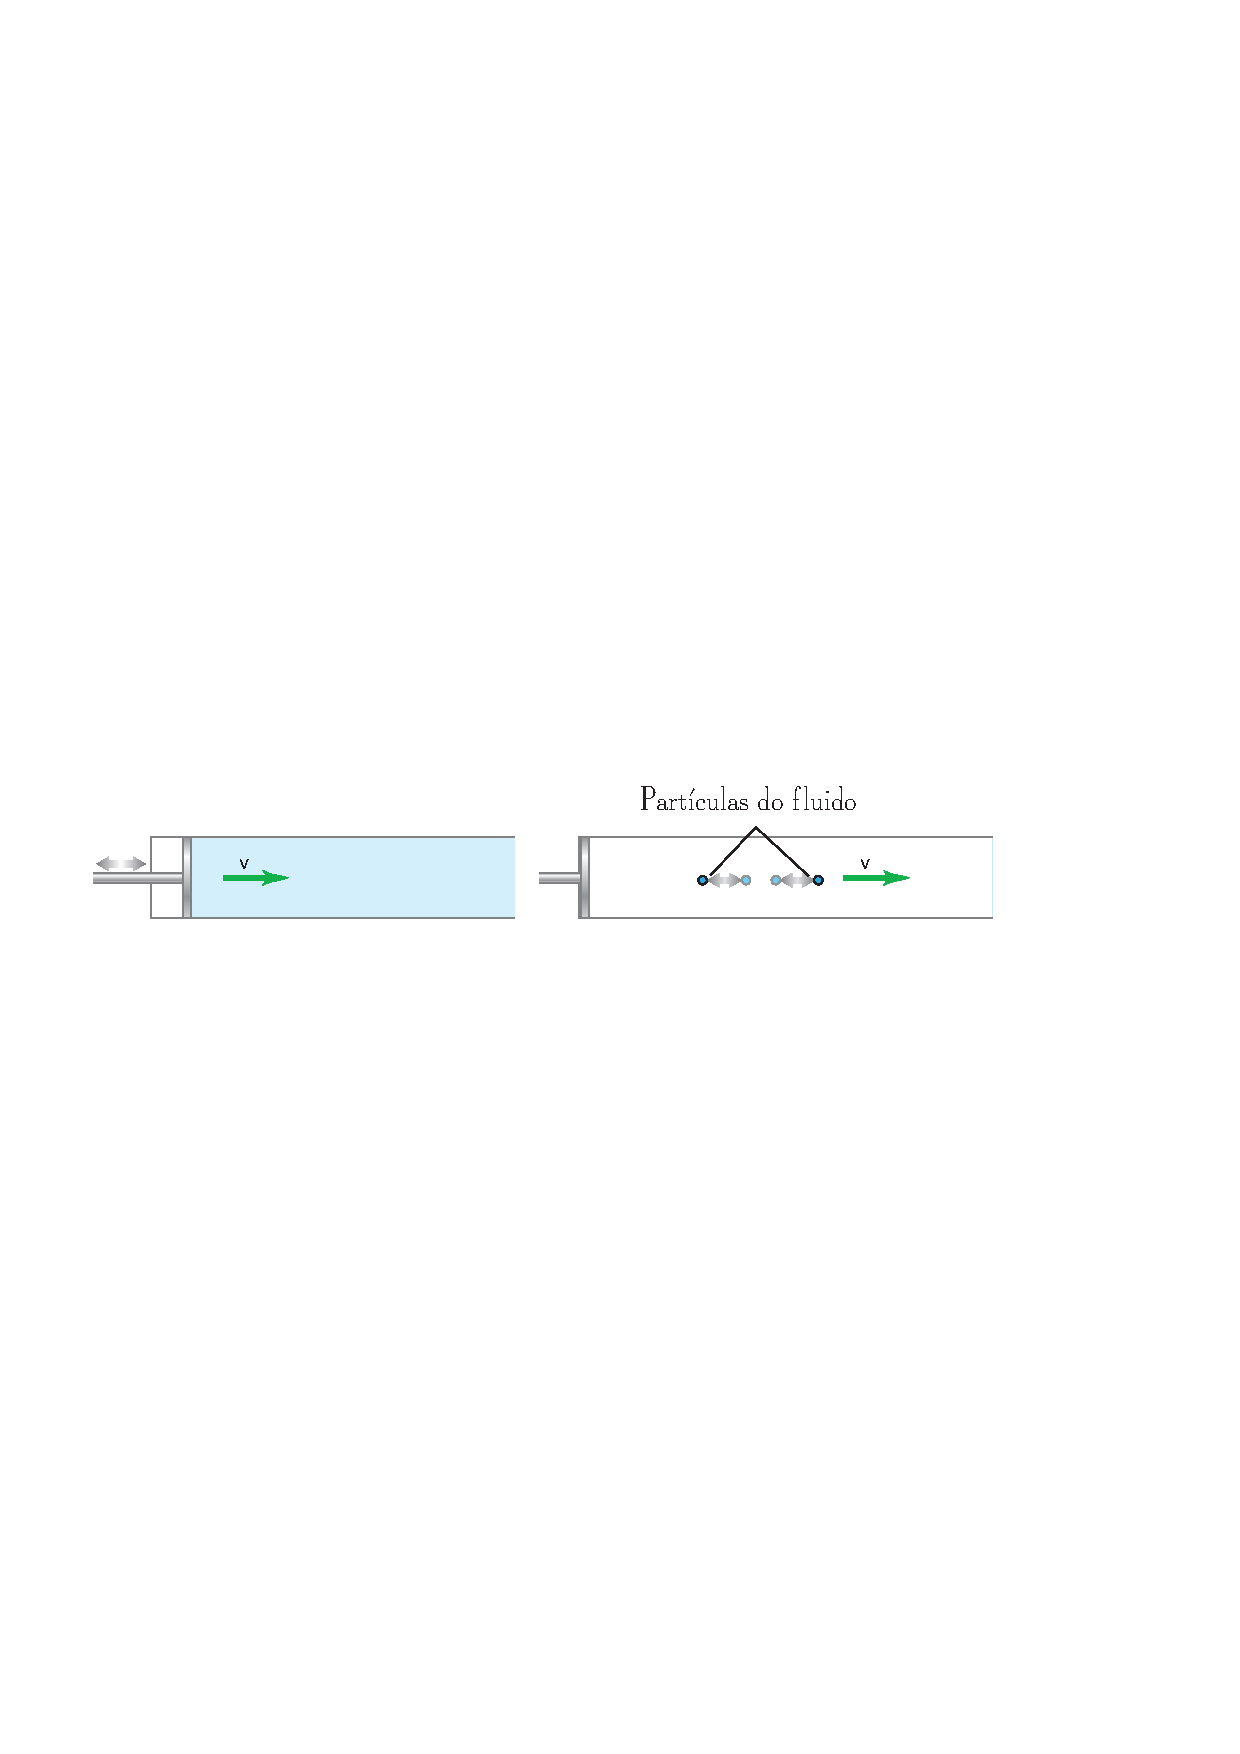
\includegraphics[scale=0.65]{images/img-2.pdf}
    \end{center}
    \legend{Fonte: extraído de \cite{young}.}
  \end{figure}
\end{itemize} 

Segundo a definição mais geral, o \textbf{som} é uma onda longitudinal em um meio. Embora capaz de propagar-se através de meio sólido, líquido ou gasoso, o \textit{ar} é o meio mais usual para se estudar conceitos sobre o som \cite{young}.

Todos os sons que escutamos, são vibrações se propagando através do ar, onde um objeto vibrador comprime as móleculas de ar (comprimindo-as juntas) e depois as espalha (lançando-as a uma certa distância). Mesmo com as flutuações na pressão, as moléculas de ar tendem a se manter na mesma posição, em média \cite{soundtrack}. 

Essas rápidas e súbitas mudanças na pressão do ar, fazem vibrar o tímpano, e assim sinais nervosos são enviados ao cérebro e interpretados como som \cite{soundtrack}.

\begin{figure}[!htb]
  \caption{\label{fig_diapasao}Diapasão: um objeto simples capaz de criar sons.}
  \begin{center}
  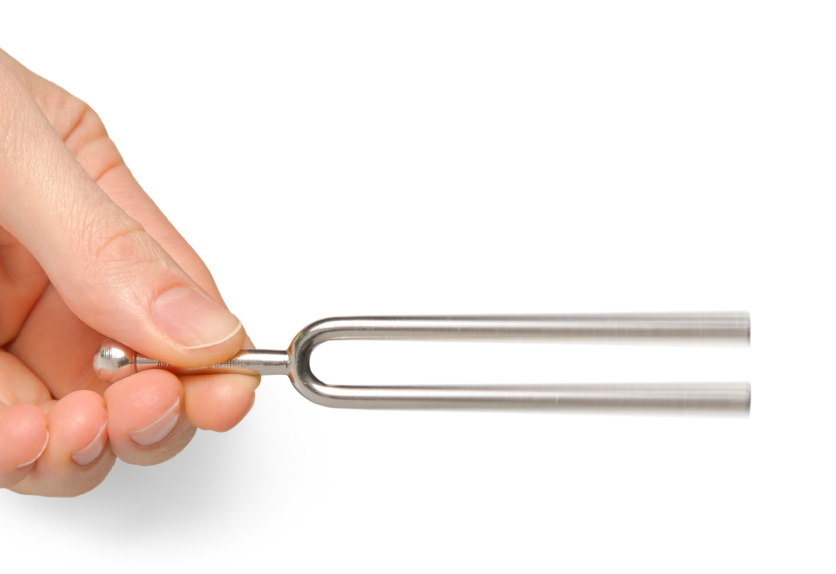
\includegraphics[scale=0.17]{images/tuning-fork.jpg}
  \end{center}
  \legend{Fonte: extraído de \cite{woman}.}
\end{figure}

Um exemplo de objeto simples capaz de criar som e demonstrar seu conceito, é o \textit{diapasão}. A medida que as pontas vibram para frente e para trás, elas empurram as partículas de ar ao seu redor.

O movimento das pontas para frente, empurram as moléculas de ar para a direita, e o recuo cria uma área de menor pressão, permitindo que as partículas sejam movidas de volta para a esquerda.

É importante ressaltar que o som \textit{não é} uma onda \textit{transversal} e sim \textit{longitudinal}, criada pelas compressões e rarefações de ar.

Como se pode ver na Figura \ref{fig_pressao}, utilizando-se o diapasão como exemplo, podemos mostrar uma \textit{representação do som por uma onda transversal senoidal}, com o intuito de ilustrar a natureza senoidal das flutuações de pressão no tempo. 

\begin{figure}[!htb]
  \caption{\label{fig_pressao}Ilustração de uma onda sonora, ou onda de pressão.}
  \begin{center}
  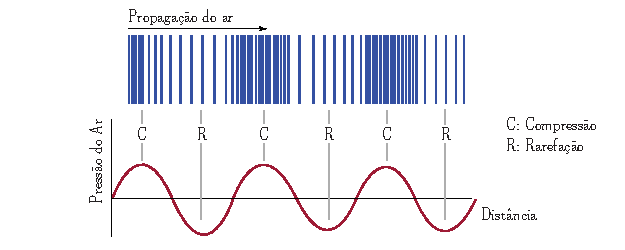
\includegraphics[scale=1.34]{images/img-3.pdf}
  \end{center}
  \legend{Fonte: extraído de \cite{class}.}
\end{figure}

% ----------------------------------------------------------
% CARACTERÍSTICAS DO SOM E DA ESCALA DECIBEL
% ----------------------------------------------------------
\section{Características do Som}\label{caracteristicas}

Dentre propriedades que caracterizam uma onda sonora, as duas consideradas mais importantes são: \textit{frequência} e \textit{amplitude}.

 Uma das formas mais simples de onda é a \textit{onda senoidal}. Embora ondas puramente senoidais sejam raramente encontradas na natureza, uma simples onda senoidal demonstra claramente estes conceitos, uma vez que todos os outros sons podem ser considerados como combinações de ondas senoidais \cite{soundtrack}.

\begin{figure}[!htb]
  \caption{\label{senoide}Exemplo de uma onda senoidal.}
  % \begin{center}
  % \includegraphics[scale=0.4]{images/sine-wave.png}
  % \end{center}
  \begin{center}
    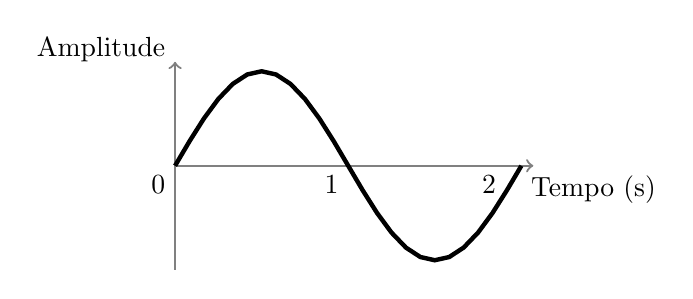
\begin{tikzpicture}[xscale=.7, yscale=1.2]
        \draw [help lines,thick, ->] (0,0) -- (6.5,0);
        \node [below right] at (2*pi,0) {Tempo (s)};
        \node [below left] at (0,0) {$0$};
        \node [below left] at (pi,0) {$1$};
        \node [below left] at (6,0) {$2$};
        \node [above left] at (0,1) {Amplitude};
        \draw [help lines, thick, ->] (0,-1.1) -- (0,1.1);
        \draw [ultra thick, blue, domain=0:2*pi] plot (\x, {sin(\x r)});
        % \draw [dashed, blue,domain=0:2*pi] plot (\x, {(sin(1.5*\x r)});
        % \draw [dashed, blue,domain=0:2*pi] plot (\x, {(sin(0.5*\x r)});
      \end{tikzpicture}
  \end{center}
  \legend{Fonte: extraído de \cite{soundtrack}.}
\end{figure}

\subsection{Frequência de um Som}

Como mencionado anteriormente, uma onda sonora é definida como uma onda de pressão que se propaga por um meio. Ao propagar-se pelo ar, a pressão atmosférica varia periodicamente.

Logo, a \textit{frequência} de um som é definida como o número de variações de pressão por segundo, e é medida em \textit{Hertz} (Hz), ou número de ciclos por segundo.

% Quanto maior a frequência (ou ciclos por segundo), mais agudo o som. Por exemplo, o som produzido por um apito (alta frequência), é mais agudo que o som produzido por um baixo elétrico (baixa frequência). 

O som que escutamos é geralmente radiado em todas as direções, a partir de um meio vibrante, e é uma combinação de muitas frequências diferentes como se pode ver na Figura \ref{complexos}.

\begin{figure}[!htb]
  \caption{\label{complexos}Os sons que ouvimos são geralmente uma mistura de frequências.}
  \begin{center}
    %\includegraphics[scale=0.3]{images/complex-sounds.png}
    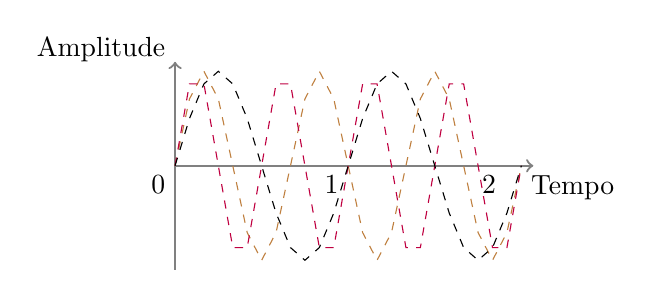
\begin{tikzpicture}[xscale=.7, yscale=1.2]
        \draw [help lines,thick, ->] (0,0) -- (6.5,0);
        \node [below right] at (2*pi,0) {Tempo};
        \node [below left] at (0,0) {$0$};
        \node [below left] at (pi,0) {$1$};
        \node [below left] at (6,0) {$2$};
        \node [above left] at (0,1) {Amplitude};
        \draw [help lines,thick, ->] (0,-1.1) -- (0,1.1);
        %\draw [blue, domain=0:2*pi] plot (\x, {sin(\x r)});
        \draw [dashed, brown,domain=0:2*pi] plot (\x, {(sin(3*\x r)});
        \draw [dashed, purple,domain=0:2*pi] plot (\x, {(sin(4*\x r)});
        \draw [dashed, black,domain=0:2*pi] plot (\x, {(sin(2*\x r)});
      \end{tikzpicture}
  \end{center}
  \legend{Fonte: extraído de \cite{control}.}
\end{figure}

Um ser humano jovem e saudável consegue escutar uma faixa de frequência de 20 Hz a 20.000 Hz. Na meia idade, esta faixa muda para 70 a 14.000 Hz. Um instrumento como o piano, tem uma faixa de 31.5 Hz a 8.000 Hz \cite{control}. Ou seja, o ser humano consegue escutar uma enorme variedade de sons. 

\subsection{Amplitude de um Som}

Uma outra propriedade do som é a sua amplitude. Quanto maior for a amplitude da pressão, maior a altura percebida do som \cite{halliday}. Sons podem possuir amplitudes diferentes, mesmo se possuírem a mesma frequência como mostra a Figura \ref{amplitude}.

\begin{figure}[!htb]
  \caption{\label{amplitude}Dois sons podem ter a mesma frequência e diferentes amplitudes.}
  \begin{center}
    %\includegraphics[scale=0.3]{images/amplitude.png}
    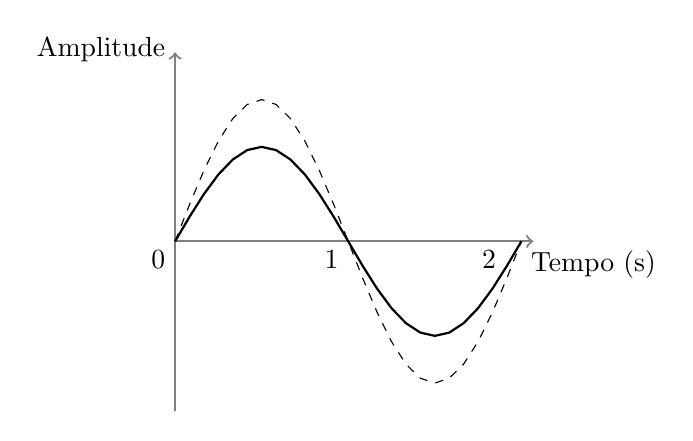
\begin{tikzpicture}[xscale=.7, yscale=1.2]
        \draw [help lines,thick, ->] (0,0) -- (6.5,0);
        \node [below right] at (2*pi,0) {Tempo (s)};
        \node [below left] at (0,0) {$0$};
        \node [below left] at (pi,0) {$1$};
        \node [below left] at (6,0) {$2$};
        \node [above left] at (0,1.8) {Amplitude};
        \draw [help lines,thick, ->] (0,-1.8) -- (0,2);
        \draw [thick, blue, domain=0:2*pi] plot (\x, {sin(\x r)});
        \draw [dashed, blue, domain=0:2*pi] plot (\x, {1.5*sin(\x r)});
        % \draw [dashed, blue,domain=0:2*pi] plot (\x, {(sin(1.5*\x r)});
        % \draw [dashed, blue,domain=0:2*pi] plot (\x, {(sin(0.5*\x r)});
    \end{tikzpicture}
  \end{center}
  \legend{Fonte: extraído de \cite{control}.}
\end{figure}

Um som de maior amplitude possui uma maior variação de pressão do que um som de menor amplitude. Define-se a \textbf{pressão} $p$ em um certo ponto, como sendo a força normal por unidade de área, ou seja, a razão entre $dF$ e $dA$ \cite{young}:

 \begin{align}
  % 1 \ pascal \ & = 1 \ Pa \ = 1 \ N/m^2
  p = \frac{dF}{dA} 
 \end{align}

Caso a pressão seja a mesma em todos os pontos de uma superfície plana finita com área $A$, então:

\begin{align}
  % 1 \ pascal \ & = 1 \ Pa \ = 1 \ N/m^2
  p = \frac{F}{A} 
\end{align}

onde $F$ é a força normal em um lado da superfície. 

A unidade utilizada para expressar pressão e variação de pressão é o \textit{Pascal} (Pa), em homenagem ao cientista e filósofo francês Blaise Pascal.
\begin{align}
   1 \ pascal \ & = 1 \ Pa \ = 1 \ N/m^2
\end{align}

O ouvido humano consegue perceber uma faixa muito ampla de pressões sonoras, sendo $20 \ \mu Pa \ (20 \cdot 10^{-6} Pa)$ o valor de pressão do som mais suave que um humano pode detectar. Este valor é chamado de \textbf{limiar da audição}. 

Em algumas situações, como no caso de um lançamento de uma nave espacial, são produzidos valores de pressão sonora de aproximadamente $200.000.000 \ \mu Pa $.%$\ (2 \cdot 10^{9} \ \mu Pa)$. 

\begin{table}[!htb]
    \caption{Relação de sons comuns em termos de pressão em $Pa$. }
    \label{tabela-pa}
    \center
    \begin{tabular}{|r|l|}
    \hline
      \rowcolor[gray]{.9}
      \textbf{Fonte do Som} & \textbf{Pressão do Som (em $\mu Pa$)}\\
      \hline
      \textsf{Lançamento de nave espacial} & \textsf{200.000.000}\\
      \hline
      \textsf{Orquestra Completa} & \textsf{20.000.000}\\
      \hline
      \textsf{Trem a \textit{diesel} em alta velocidade a 25 metros} & \textsf{200.000}\\
      \hline
      \textsf{Conversa normal} & \textsf{20.000}\\
      \hline
      \textsf{Cochicho suave a 2 metros} & \textsf{2.000}\\
      \hline
      \textsf{Sala de transmissão vazia} & \textsf{200}\\
      \hline
      \textsf{Limiar da audição humana} & \textsf{20}\\
      \hline
    \end{tabular}
  \end{table}

Como se pode ver na Tabela \ref{tabela-pa}, lidar com números que variam tanto quanto os valores de pressão sonora em $Pa$, é uma tarefa incoviniente (de 20 a 2.000.000.000). 

Uma maneira mais simples é utilizar a \textit{Escala Logarítmica}, que é a base para a \textit{Escala Decibel}, discutida na Seção \ref{escala-db}.

\section{A Escala Decibel}\label{escala-db}

Como visto na seção acima, a aplicação direta de uma escala linear para medir pressão sonora, em $Pa$, levaria ao uso de números enormes. No entanto, utilizando-se de uma escala logarítmica, podemos representar tais valores altos em menores, tornando a manipulação mais simples como vemos na Figura \ref{log}. 

\begin{figure}[!htb]
  \caption{\label{log}Função $y=log_{10}x$ e alguns valores de demonstração.}
  \begin{center}
    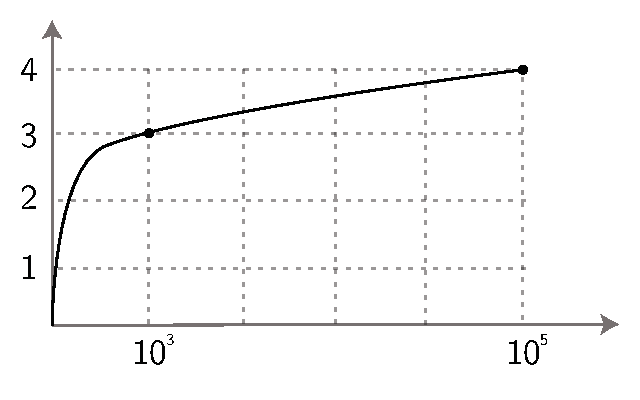
\includegraphics[scale=0.6]{images/log.pdf}
    % \begin{tikzpicture}
    %   \begin{axis}[
    %       axis x line=middle, 
    %       axis y line=middle, 
    %       ymax=0.1E8, ylabel=$y$, 
    %       xlabel=$x$
    %       ]
    %   \addplot[domain=-10000:10000, blue, ultra thick] {14*x - x^2};
    %   \end{axis}
    % \end{tikzpicture}
  \end{center}
  \legend{Fonte: extraído de \cite{xing}.}
\end{figure}

Além do mais, nossos ouvidos não respondem a estímulos de maneira linear, e sim logarítmica. Logo, percebe-se que é mais prático expressar valores de pressão sonora a partir de uma proporção logarítmica de um valor medido com um valor de referência. Esta proporção logarítmica é chamada de \textbf{decibel} ou \textbf{dB}, em homenagem ao trabalho de Alexander Graham Bell, o inventor do telefone \cite{young}.

\begin{figure}[!htb]
  \caption{\label{escala}A conviniência da Escala Decibel.}
  \begin{center}
    %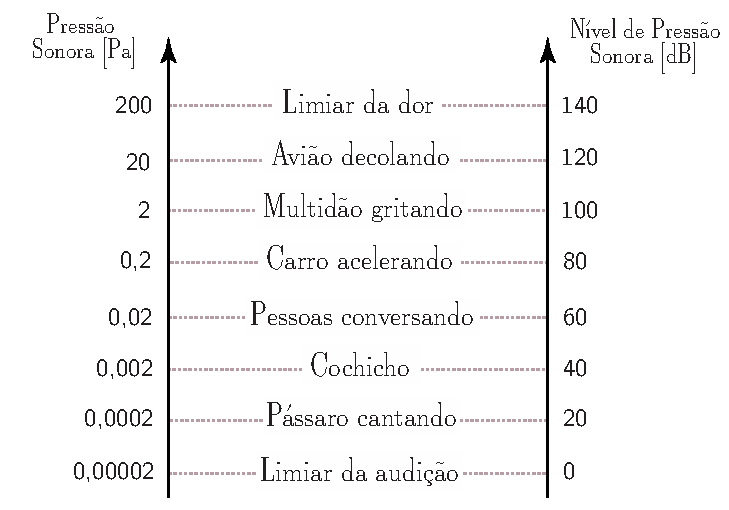
\includegraphics[scale=0.38]{images/escala.png}
    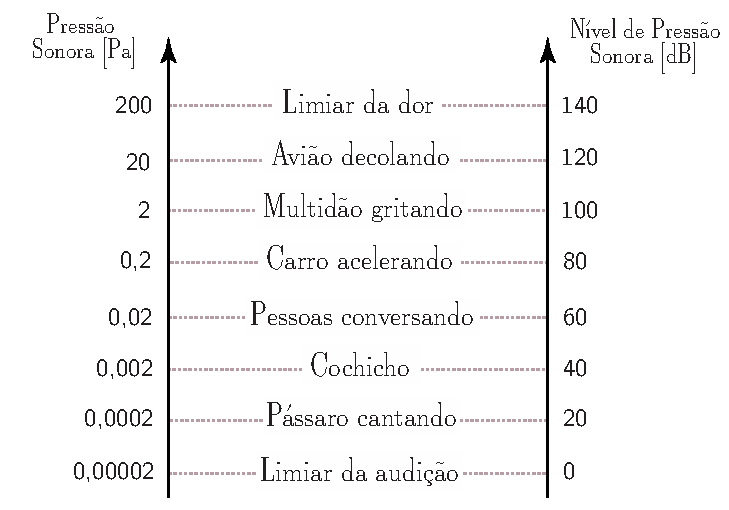
\includegraphics[scale=0.9]{images/escala.pdf}
  \end{center}
  \legend{Fonte: extraído de \cite{bojo}.}
\end{figure}

É importante frisar que o decibel \textit{não é} uma unidade para medir som, e sim uma medida \textit{relativa} \cite{water}. Em termos de nível de pressão sonora em decibéis, tem-se o limiar da audição como sendo 0 dB e o limiar da dor como sendo 130 dB, como se pode ver na Figura \ref{escala}. Em certas situações, pode ocorrer rompimento do tímpano com valores em cerca de 190 dB.

Portanto, o valor de \textit{Nível de Pressão Sonora} em decibéis, abreviado para \textit{SPL} (\textit{Sound Pressure Level}) ou $L_p$ (\textit{Level of pressure}), é obtido pela fórmula:

\begin{align}\label{eq-dec}
  SPL \ = \ 20\cdot log_{10} \left(\frac{p}{p_0}\right)
\end{align}

sendo $p$ (RMS) o valor medido em $Pa$, e $p_0$ (RMS) o valor de referência padrão que é de $20 \ \mu Pa$ -- limiar da audição humana. 

Segundo a \textit{Brüel \& Kjær}, empresa multinacional e maior fabricante e fornecedora de equipamentos de medição de som e vibração, embora existam outros parâmetros do som que podem ser medidos como intensidade e potência, em casos de avaliação de nocividade e incômodo de fontes sonoras (que é o caso deste trabalho), o fator importante a se considerar é a \textit{pressão sonora} \cite{bojo}.

\section{Como medir Níveis Sonoros}

\subsection{Medidor de Nível de Pressão Sonora (MNPS)}

O instrumento utilizado para medir níveis de pressão sonora é chamado de \textit{Medidor de Nível de Pressão Sonora} (MNPS), ou mais conhecido por \textit{Decibelímetro}. 

Um MNPS trata-se de um instrumento projetado para responder ao som de maneira semelhante ao ouvido humano, e reproduzir medidas de níveis de pressão sonora.


\begin{figure}[!htb]
  \caption{\label{decib} Medidor de Nível de Pressão Sonora Comum (ou \textit{Decibelímetro}).}
  \begin{center}
  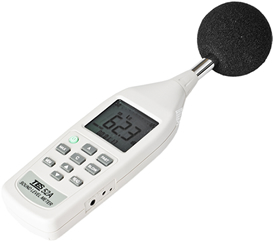
\includegraphics[scale=1.1]{images/decibelimetro.jpg}
  \end{center}
  \legend{Fonte: extraído de \cite{decib}.}
\end{figure}

Embora exista uma infinidade de aparelhos como este, que diferem em detalhes, todos compartilham de um sistema que consiste em um microfone, um circuito processador do sinal captado, e uma unidade de leitura.

Detalhadamente, algumas etapas que envolvem as etapas de um Medidor de Níveis de Pressão Sonora são:

\begin{enumerate}
  \item Um microfone que é utilizado para captar o som e convertê-lo em um sinal elétrico equivalente;
  \item Após a leitura e conversão do som em sinal elétrico, um circuito \textit{pré-amplificador} entra em ação para amplificar (aumentar a amplitude) o sinal, devido ao sinal gerado pelo microfone ser de baixa amplitude.
  \item Com o sinal amplificado, vários tipos de processamento podem ser aplicados, sendo o mais comum a aplicação de um \textit{filtro de ponderação A};
  \item \textit{Display} de saída de dados.
\end{enumerate}

\begin{figure}[!htb]
  \caption{\label{diag-blocos}Diagrama de blocos de um Medidor de Nível de Pressão Sonora Básico.}
  \begin{center}
  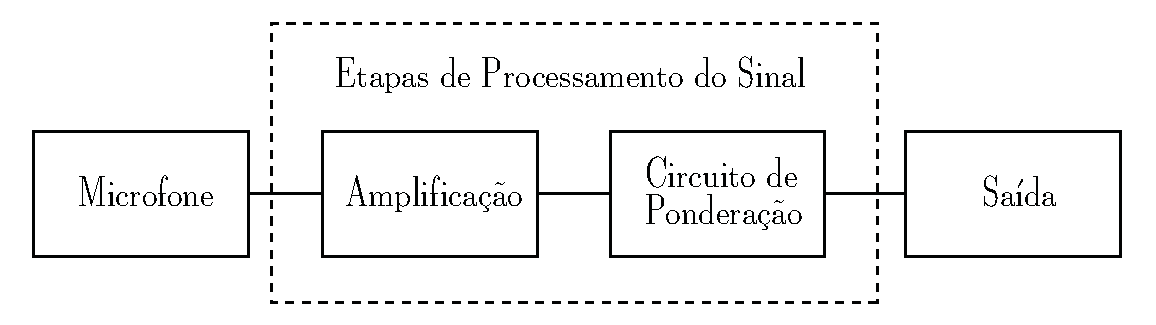
\includegraphics[scale=0.65]{images/etapas.pdf}
  \end{center}
  \legend{Fonte: o autor.}
\end{figure}

\subsection{Curva de Ponderação A}

No ano de 1933, os pesquisadores Fletcher e Munson publicaram um conjunto de curvas mostrando a sensibilidade do ouvido humano a amplitude de um som, comparado a sua frequência. 

Essas curvas mostravam que o ouvido humano é mais sensível a sons que possuem uma frequência entre 3000-4000 Hz. Sons com frequências abaixo ou acima desta faixa devem possuir uma amplitude maior para serem igualmente altos como se pode ver na Figura \ref{fletcher}.

Alguns anos depois desta publicação, tais curvas foram utilizadas no primeiro padrão \textit{American National Standars Institute} (ANSI) para medidores sonoros, o qual incorporou a curva de ponderação A e B (esta logo caiu em desuso).

A curva de ponderação A é a mais frequentemente utilizada para medição sonora pois é a que mais reflete verdadeiramente a maneira como os seres humanos escutam (atenuando somente as frequências audíveis).

\begin{figure}[!htb]
  \caption{\label{fletcher}Curvas de Fletcher–Munson: relação frequência-amplitude do ouvido.}
  \begin{center}
  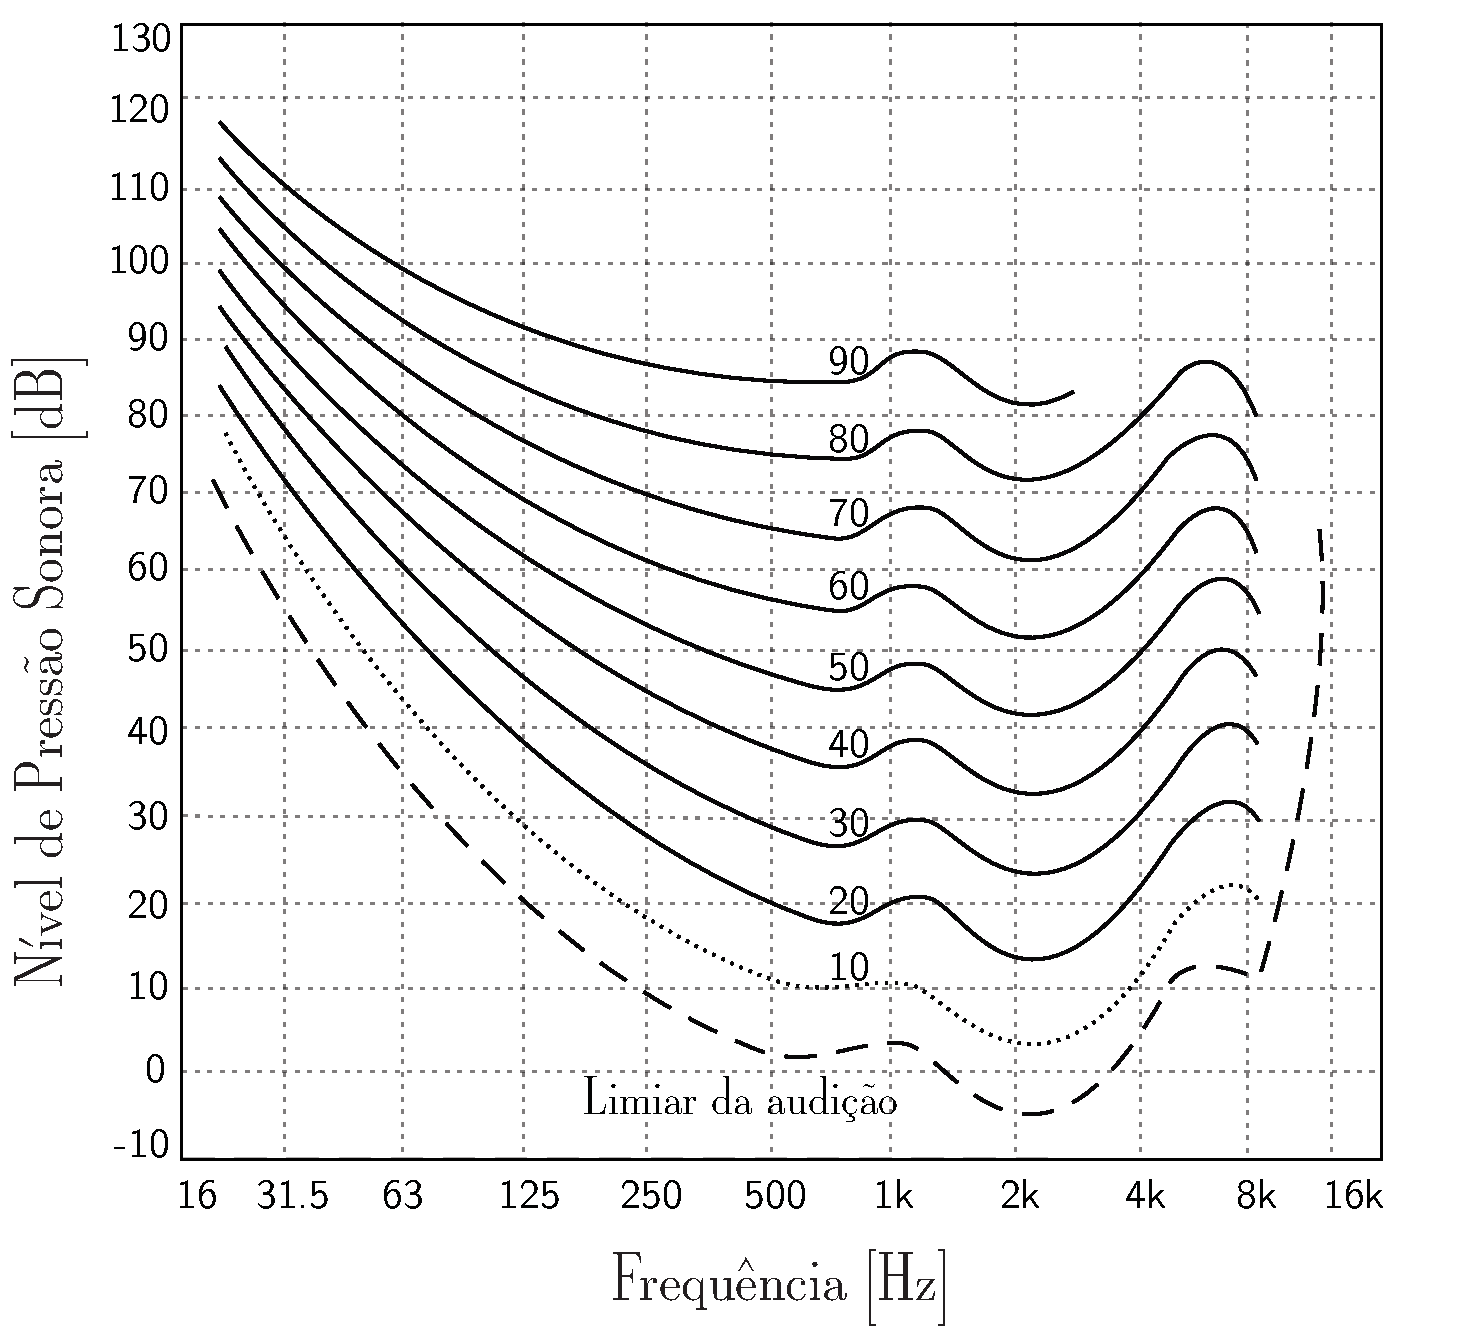
\includegraphics[scale=0.33]{images/fletcher.pdf}
  \end{center}
  \legend{Fonte: extraído de \cite{manson}.} %http://replaygain.hydrogenaud.io/proposal/pics/equal_loudness.gif
\end{figure}

Como se pode ver na Figura \ref{a-weight}, a Curva de Ponderação A cobre o intervalo inteiro de frequências de 10 Hz a 10kHz. No entanto, o formato dela se aproxima das frequências percebidas pelo ouvido humano.

\begin{figure}[!htb]
  \caption{\label{a-weight}Filtro de ponderação A.}
  \begin{center}
  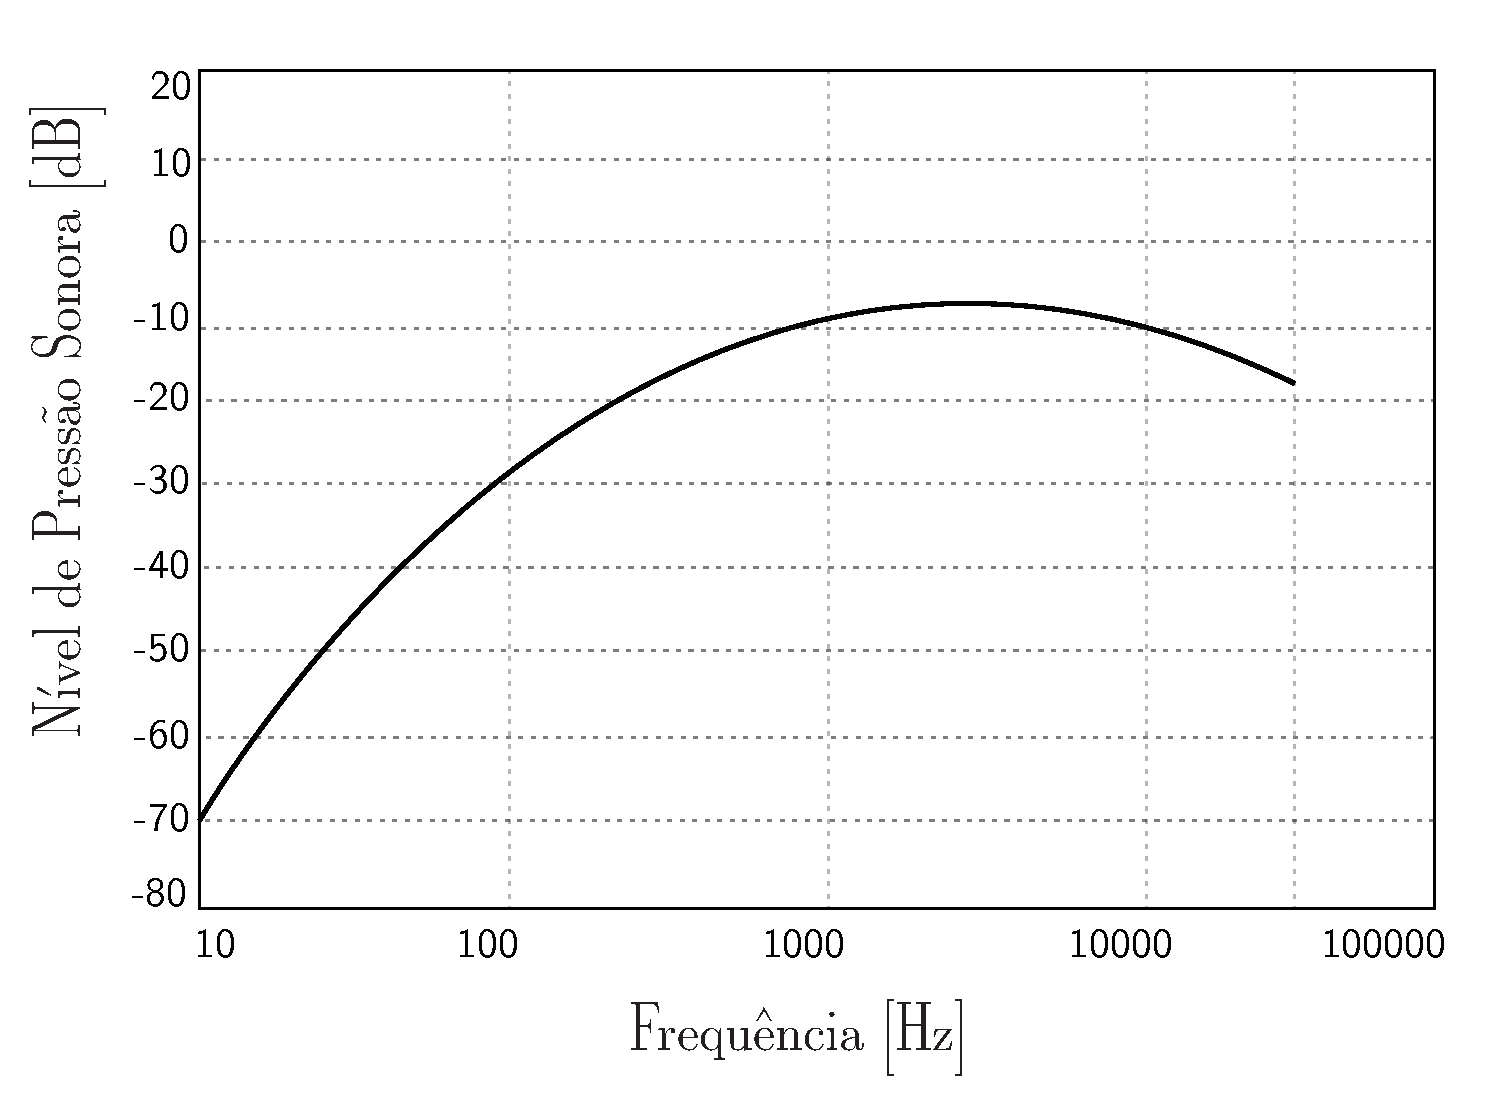
\includegraphics[scale=0.32]{images/a-weight.pdf}
  \end{center}
  \legend{Fonte: extraído de \cite{weight}.} %http://replaygain.hydrogenaud.io/proposal/pics/equal_loudness.gif
\end{figure}

As medidas feitas utilizando esta curva são expressas em dB(A) para mostrar que foi utilizado uma Curva de Ponderação A no processo de medição. Nesse contexto, níveis sonoros são expressos em $L_{p(A)}$.

\subsection{MNPS Integrador}

Como citado na Seção anterior, um MNPS comum é capaz de medir a amplitude de um som em determinado momento. 

Porém, isto pode não ser algo muito útil quando é necessário tirar uma média dos níveis sonoros de um ambiente por um certo espaço de tempo, uma necessidade comum para fábricas, por exemplo, que necessitam monitorar a intensidade do ruído das máquinas.

\begin{figure}[!htb]
  \caption{\label{integ}Medidor de Nível de Pressão Sonora Integrador.}
  \begin{center}
    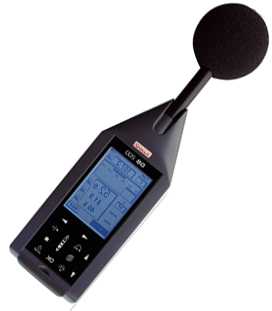
\includegraphics[scale=0.34]{images/integrador.jpg}
  \end{center}
  \legend{Fonte: extraído de \ref{decib}.} %http://www.kimocanada.com/Images/db200.jpg
\end{figure}

Para esta tarefa, o instrumento utilizado é um pouco mais sofisticado (e caro) que um MNPS comum, e se chama \textit{Medidor de Nível de Pressão Sonora Integrador}, onde a palavra \textit{integrador} diz respeito a soma dos valores durante um período de tempo. 

Além do mais, muitos deles também possuem um \textit{data-logger} interno, capaz de gerar gráficos e dados estatísticos a respeito dos valores de pressão sonora obtidos por determinados períodos de tempo.

\chapter{Desenvolvimento do Sistema}\label{projeto}

Este capítulo busca explicar os passos que envolveram a criação e desenvolvimento tanto do projeto do medidor em \textit{hardware} quanto do \textit{software} monitorador dos valores de níveis sonoros. Na Seção \ref{proj-hard}, são exibidos os componentes utilizados e suas conexões. Na Seção \ref{comp-ut}, cada um dos componentes utilizados no projeto são detalhados e são detalhados os motivos para sua utilização.

Já na Seção \ref{montagem}, um passo-a-passo é desenvolvido, indo desde as primeiras conexões da placa até o projeto final na \textit{protoboard}.

Ao final do capítulo, na Seção \ref{projeto-soft}, são explicitadas as principais ferramentas usadas para o  desenvolvimento do \textit{software} para iOS, bem como telas e detalhamento a respeito de sua utilização para monitoramento remoto.

\section{Projeto do \textit{Hardware}}\label{proj-hard}

Como já mencionado anteriormente, um MNPS Integrador é uma ferramenta cara, tornando ainda mais cara a compra de vários aparelhos para monitorar constantemente os níveis de pressão sonora em ambientes. 

Neste contexto, o projeto de \textit{hardware} aqui apresentado trata-se de uma solução de baixo custo, com possibilidade de monitoramento \textit{online} via \textit{software}, das estações que tiverem o dispositivo instalado.

\begin{figure}[!htb]
  % \begin{center}
  % \includegraphics[scale=0.4]{images/sine-wave.png}
  % \end{center}
  \begin{center}
    \caption{\label{sistema}Diagrama de blocos ilustrando o \textit{hardware} do medidor e seus componentes.}
    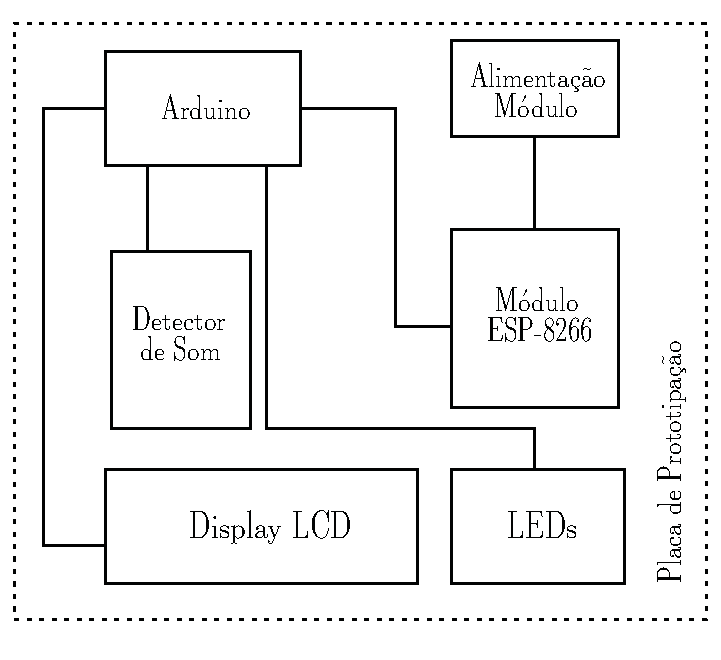
\includegraphics[scale=0.68]{images/sistema.pdf}
  \end{center}
  \legend{Fonte: o autor.}
\end{figure}

\section{Componentes Utilizados}\label{comp-ut}

A Figura \ref{sistema} ilustra as conexões entre os componentes utilizados e as próximas Seções descrevem cada um deles, detalhando suas funcionalidades e motivos que levaram a sua escolha nesta aplicação.

\subsection{O Arduino}

\textit{Arduino} é um plataforma de desenvolvimento de microcontrolador com uma linguagem de programação intuitiva que pode ser utilizada com o \textit{Arduino} \textit{Integrated Development Environment} (IDE), a partir do qual programas podem ser escritos e gravados no microcontrolador embutido na placa.
%citar exploring arduino

\begin{figure}[!htb]
  \begin{center}
    \caption{\label{arduino}\textit{Arduino UNO} e componentes: plataforma de desenvolvimento.}
    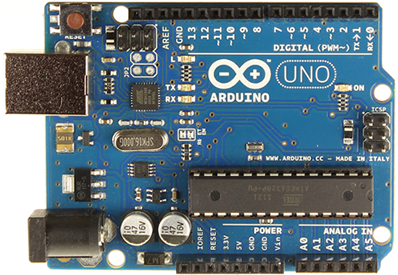
\includegraphics[scale=0.35]{images/arduino2.jpg}
  \end{center}
  \legend{Fonte: exploring arduino.}
\end{figure}

Toda a família de placas \textit{Arduino} possui um conjunto básico de funcionalidades que incluem:

\begin{itemize}
  \item Microcontrolador \textit{Atmel} ;
  \item LEDs de \textit{debug} e serial \textit{TX/RX};
  \item Interfaces de programação/comunicação USB;
  \item Pinos de Entrada/Saída;
  \item Reguladores de tensão e conexões de energia;
  \item Conectores \textit{In-Circuit Serial Programmer} (ICSP);
\end{itemize}
%citar arduino cookbook

Na Figura \ref{arduino} v\^e-se alguns detalhes do modelo de \textit{Arduino} utilizado para o desenvolvimento deste projeto e seus componentes nomeados.

Ao conectar sensores, atuadores, auto-falantes, módulos ou algum tipo de circuito integrado aos pinos de entrada/saída do Arduino, o mesmo pode se tornar uma poderosa ferramenta para controlar basicamente qualquer sistema, com um custo extremamente baixo. 

Um fato importante a mencionar é que o Arduino é um \textit{open-source hardware}. Isto significa que esquemáticos, código fonte e arquivos de projeto estão todos disponíveis gratuitamente.

\subsection{Módulo ESP8266}

O Módulo ESP8266 trata-se de uma pequena placa projetada pela \textit{Espressif Systems}, uma companhia Chinesa com sede em Shanghai.

Como descrito em sua documentação, o ESP8266 é uma solução de rede \textit{WiFi} que pode ser utilizada como ponte com microcontroladores para adicionar a capacidade de Internet.

\begin{figure}[!htb]
  \begin{center}
    \caption{\label{esp-mod}Módulo ESP8266 Versão 1.}
    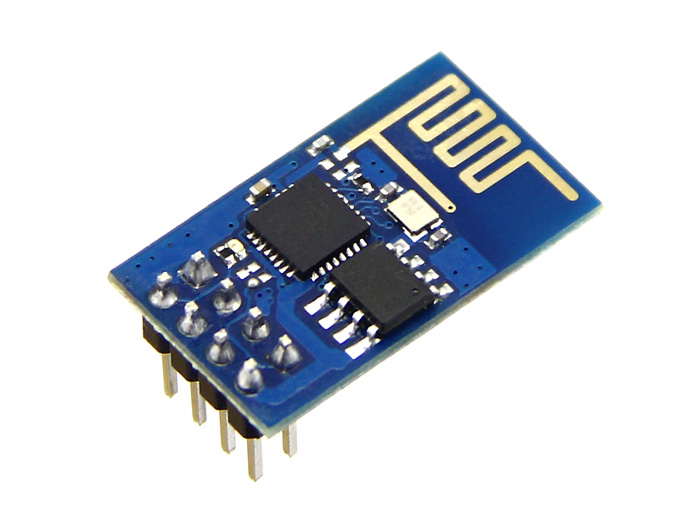
\includegraphics[scale=0.22]{images/esp.jpg}
  \end{center}
  \legend{Fonte: extraído de \cite{chip-esp}.} %http://tecdev.com.br/wp-content/uploads/2015/05/WiFi-Serial-Transceiver-Module.jpg
\end{figure}

Por conter um microprocessador, portas de entrada e saída, memória RAM (\textit{Random Access Memory}) e \textit{flash}, este poderoso módulo dispensa até mesmo a necessidade de utilizar um microcontrolador externo, podendo rodar programas de maneira independente. 

Em suma, trata-se de um microprocessador alternativo que possui suporte a WiFi e TCP/IP (\textit{Transmission Control Protocol / Internet Protocol}) embutidos, por um valor semelhante ao de um \textit{Arduino}.

\begin{figure}[!htb]
  \begin{center}
    \caption{\label{esp-chip}\textit{Chip} ESP8266 da \textit{Espressif}.}
    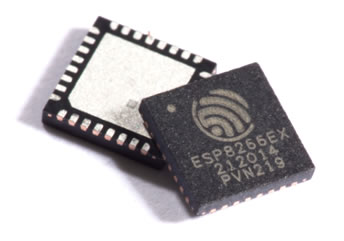
\includegraphics[scale=0.4]{images/esp-chip-2.jpg}
  \end{center}
  \legend{Fonte: extraído de \cite{chip-esp}.} %http://espressif.com/en/products/esp8266/
\end{figure}

Existem uma série de estilos de placa do ESP8266. Porém, por motivos como custo, robustez  do projeto, e disponibilidade, foi escolhida a primeira versão desta placa, a ESP-1. 

Todas as placas contém o mesmo \textit{chip} ESP8266 (Figura \ref{esp-chip}). O que difere-as são componentes como a quantidade de portas de entrada/saída, o estilo dos conectores, quantidade de memória \textit{flash} disponível e assim por diante. Algumas das especificações do \textit{chip} ESP8266 incluem:

\begin{itemize}
  \item Protocolo 802.11 b/g/n (WiFi);
  \item Pilha de protocolo TCP/IP integrada;
  \item CPU de 32-bits de baixo consumo;
  \item Consumo de energia < $1mW$ em modo \textit{standby}; 
\end{itemize}

Devido a necessidade de acesso \textit{WiFi} do projeto do medidor desenvolvido neste trabalho, outras alternativas além do Módulo ESP8266 foram consideradas. 

No entanto, devido a crescente comunidade de entusiastas do ESP e crescente fóruns de discussão, preço baixo da versão 1, tamanho do módulo, dentre outros, foi decidido utilizá-lo e integrá-lo ao \textit{Arduino UNO}, que pasou a contar com a capacidade de Internet a partir disso. 

Assim, tornaria-se possível utilizar os dados do medidor processados no \textit{Arduino}, e enviá-los para a Internet, onde o \textit{software} desenvolvido também neste trabalho, poderia então acessá-los.

Os detalhes da montagem e funcionamento são descritos na Seção \ref{montagem}.

\subsection{Detector de Som}

O detector de som \textit{SparkFun Sound Detector} é uma pequena placa produzida pela \textit{SparkFun Electronics}, uma revendedora de compononentes eletrônicos situada em \textit{Niwot, Colorado}, nos Estados Unidos. Trata-se de uma placa que combina um microfone e alguns circuitos de processamento. 

\begin{figure}[!htb]
  \begin{center}
    \caption{\label{spark}\textit{SparkFun Sound Detector}: um detector de som robusto.}
    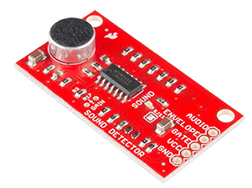
\includegraphics[scale=0.5]{images/spark.jpg}
  \end{center}
  \legend{Fonte: extraído de \cite{spark}.} %https://learn.sparkfun.com/tutorials/sound-detector-hookup-guide?_ga=1.41145250.1435560018.1439029156
\end{figure}

Em suas saídas, como se pode ver na Figura \ref{spark}, encontramos uma indicação binária da presença de som (\texttt{GATE}), sendo nível ALTO para som e nível BAIXO para silêncio, uma saída de áudio (\texttt{AUDIO}), e também uma representação analógica da amplitude do som (\texttt{ENVELOPE}). Para ligá-la, basta alimentar \texttt{VCC} e \texttt{GND}.

O valor relativamente baixo, facilidade de configuração, e principalmente a saída que representa a amplitude sonora, foram os fatores determinantes na escolha deste circuito integrado para o projeto do medidor.

\subsection{Display LCD}

Como dispositivo de saída do \textit{hardware}, foi utilizado um \textit{Liquid Crystal Display} (LCD) comum semelhante ao da Figura \ref{lcd}, de 16 colunas e 2 linhas. 

Este \textit{display} utiliza 16 pinos de conexão que incluem sinais de dados, controle e alimentação.

\begin{figure}[!htb]
  \begin{center}
    \caption{\label{lcd}\textit{Display} LCD comum: modo de saída de dados para o usuário.}
    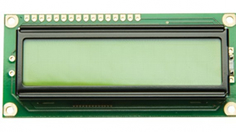
\includegraphics[scale=0.45]{images/lcd.jpg}
  \end{center}
  \legend{Fonte: extraído de \cite{lcd}.} %http://www.hobbytronics.co.uk/image/cache/data/rapid/16-2-lcd-backlight-green-2-500x500.jpg
\end{figure}

Apesar da possibilidade de monitoramento via \textit{software}, entendeu-se que seria interessante que os locais possuindo o \textit{hardware} instalado e em funcionamento, pudessem ter uma ideia do \textit{status} da medição do som instantaneamente. 

Assim, decidiu-se por incorporar tal \textit{display} para incrementar o \textit{hardware} desenvolvido.

\subsection{LEDs}

Por fim, embora o \textit{status} de monitoramento possa ser lido diretamente do \textit{display}, ou acessado via \textit{software}, existem algumas situações em que pode ser necessário verificar o \textit{status} somente olhando para o \textit{hardware} do medidor.

% \begin{figure}[!htb]
%   \begin{center}
%     \caption{\label{leds}Diodos emissores de luz (LEDs) nas cores verde, amarela e vermelha.}
%     \includegraphics[scale=0.25]{images/leds.jpg}
%   \end{center}
%   \legend{Fonte: extraído de \cite{leds}.} %http://pt.aliexpress.com/store/product/100Pcs-Round-Head-LED-Light-Emitting-Diode-Red-Green-Yellow-3mm-5mm-BS88/1213392_1975921656.html?storeId=1213392
% \end{figure}

Por este motivo, também foram utilizados os bastantes conhecidos diodos emissores de luz, \textit{Light Emitting Diode} (LED), em três diferentes cores para indicar a intensidade do som de maneira intuitiva. 

Um LED verde acesso indica uma intensidade de som \textit{baixa}, um LED amarelo indica intensidade \textit{média}, e um LED vermelho indica intensidade \textit{alta}.

\section{Montagem dos componentes}\label{montagem}

De posse dos componentes mencionados na Seção anterior, o circuito foi montado numa \textit{protoboard} MSB-500 da fabricante nacional ICEL, seguindo o diagrama de blocos da Figura \ref{sistema}.

Para facilitar a explicação das conexões feitas na \textit{protoboard}, decidiu-se separar as ligações em etapas que serão descritas a seguir e só ao final será apresentada a solução completa.

\subsection{Arduino e Detector de Som}

Como mencionado anteriormente, a saída \texttt{ENVELOPE} entrega um valor de tensão DC que corresponde ao valor de pico do sinal de entrada. 

O sinal de entrada captado pelo microfone de eletreto possui uma tensão muito pequena, por isso a primeira etapa do circuito é responsável por amplificá-lo com um ganho aritmético de $100$. Inclusive, a placa possui uma entrada para soldar um resistor (ou potenciômetro), caso seja necessário aumentar ou diminuir o ganho do amplificador. 

O circuito que entrega o valor de saída do \texttt{ENVELOPE} trata-se de um circuito \textit{Retificador de Precisão de Meia Onda} utilizando amplificador operacional. Assim, o amplificador inverte e amplifica tal sinal $V_{in}$ (Figura \ref{seg}).

Como se pode ver na Figura \ref{circ}, a única porta de saída do Detector de Som (DDS) que foi utilizada foi a \texttt{ENVELOPE}, conectada diretamente a porta de entrada analógica \texttt{A0} do \textit{Arduino}. Segundo o \textit{datasheet} do DDS, a alimentação ideal é $5V$.

\begin{figure}[!htb]
  \begin{center}
    \caption{\label{seg}Segunda etapa do circuito do DDS: seguidor de envelope.}
    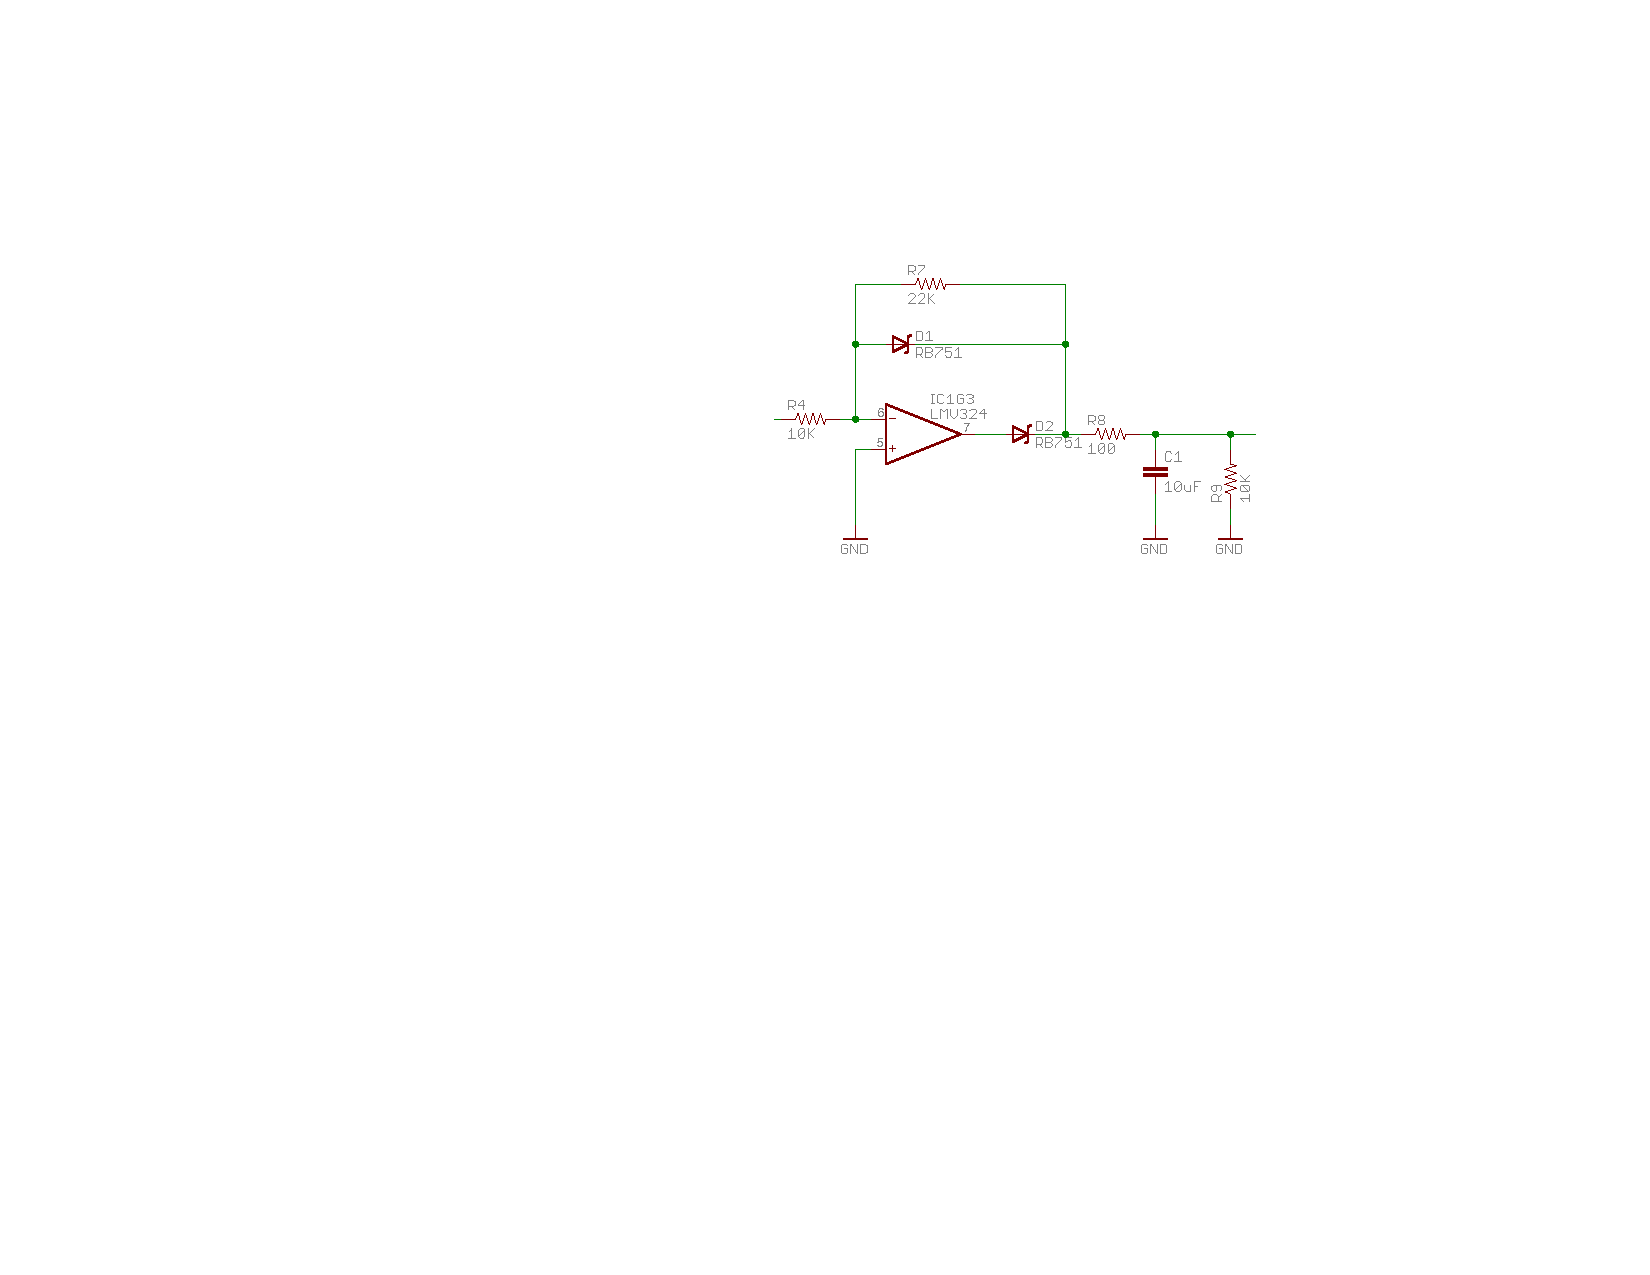
\includegraphics[scale=1.2]{images/schematic.pdf}
  \end{center}
  \legend{Fonte: extraído de \cite{spark}.} %http://www.hobbytronics.co.uk/image/cache/data/rapid/16-2-lcd-backlight-green-2-500x500.jpg
\end{figure}

O sinal $V_{in}$ é então amplificado e invertido. Quando a tensão de entrada é maior que zero, $D_2$ não está conduzindo e $D_1$ está, então a tensão de saída $V_{out}$ é zero pois um lado do $R_7$ está conectado ao terra virtual e não há corrente passando naquele ponto. 

Quando $V_{in}$ é menor que zero, $D_2$ está conduzindo e $D_1$ está como circuito aberto, e a saída é amplificada com um ganho de $\frac{-R_7}{R_4}$. 

Por fim, o capacitor $C_1$ se carrega com o valor de tensão de pico, sendo então o responsável por armazenar o maior valor de tensão do sinal de entrada. Também, $C_1$ se descarrega através de $R_9$, nos ciclos em que $D_2$ não está conduzindo.

Esta etapa do circuito implementa a equação:

\begin{figure}[!htb]
  \begin{center}
      \begin{verbatim}
                              if (Vin > 0) 
                                Vout = 0;
                              else
                                Vout = Vin * -2,2 
      \end{verbatim}
    \end{center}
\end{figure}

Onde $-2,2$ é o ganho do amplificador dado por $\frac{-R_7}{R_1} = \frac{22k\Omega}{10k\Omega} = -2,2$.

Portanto, ao efetuar as conexões do DDS com o \textit{Arduino} como visto na Figura \ref{circ}, é possível obter o valor de tensão de pico do som. 

\begin{figure}[!htb]
  \begin{center}
    \caption{\label{circ}Conexão entre \textit{Arduino} e Detector de Som.}
    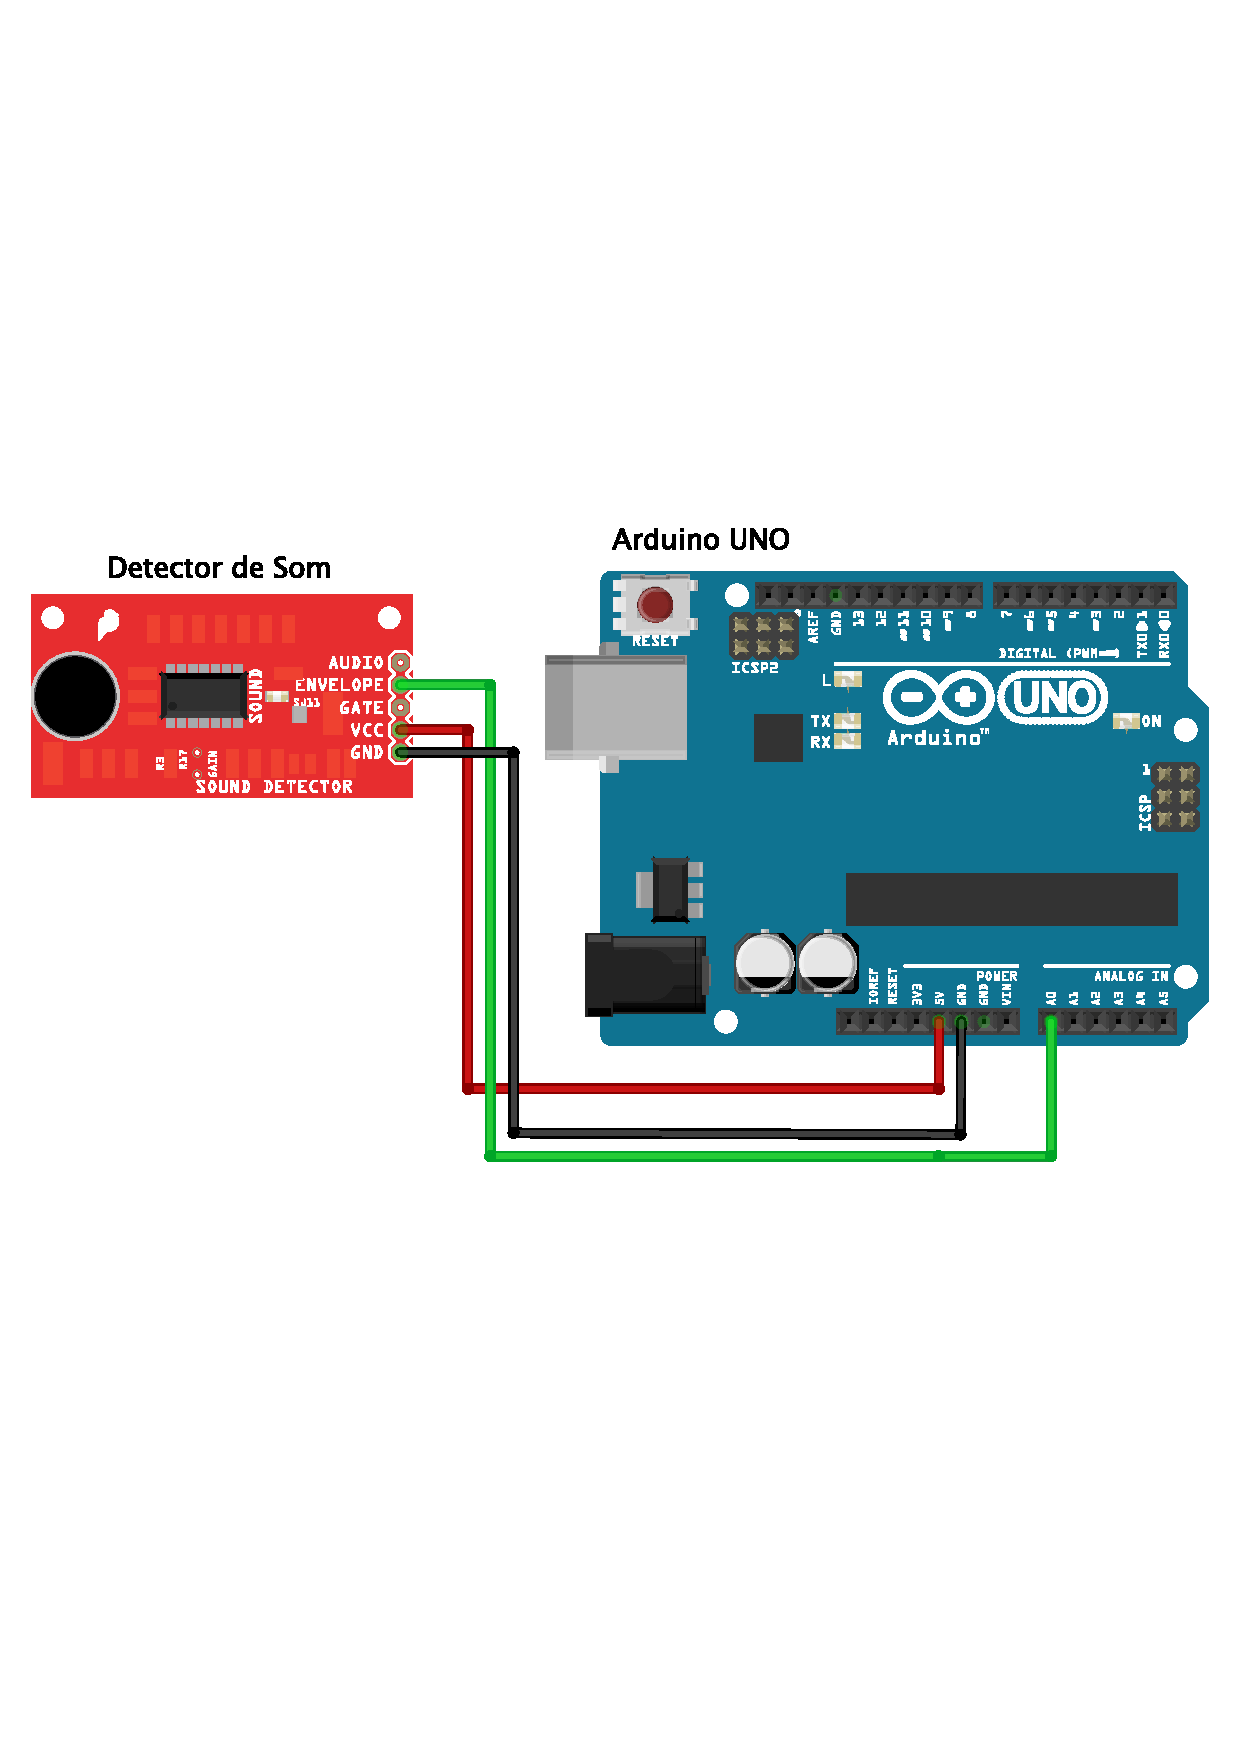
\includegraphics[scale=0.41]{images/circ-1.pdf}
  \end{center}
  \legend{Fonte: o autor.} %http://www.hobbytronics.co.uk/image/cache/data/rapid/16-2-lcd-backlight-green-2-500x500.jpg
\end{figure}

O \textit{Arduino UNO} possui um conversor analógico digital de 10 bits de resolução, o que significa que é possível representar valores de 0 a 1023 ($2^{10}=1024$). Isto significa que, para obter o valor de tensão de pico, é necessário fazer a conversão $\frac{(V_{cc}\cdot A_0)}{1024}$. 

\subsection{Arduino e ESP8266}

Para se comunicar com o Módulo ESP8266, foi utilizada a biblioteca \texttt{SoftwareSerial}, que torna possível a utilização de portas comuns do Arduino para comunicação serial com outros dispositivos. 

\begin{figure}[!htb]
  \begin{center}
    \caption{\label{circ-2}Conexão entre \textit{Arduino}, Módulo ESP8266 e Detector de Som.}
    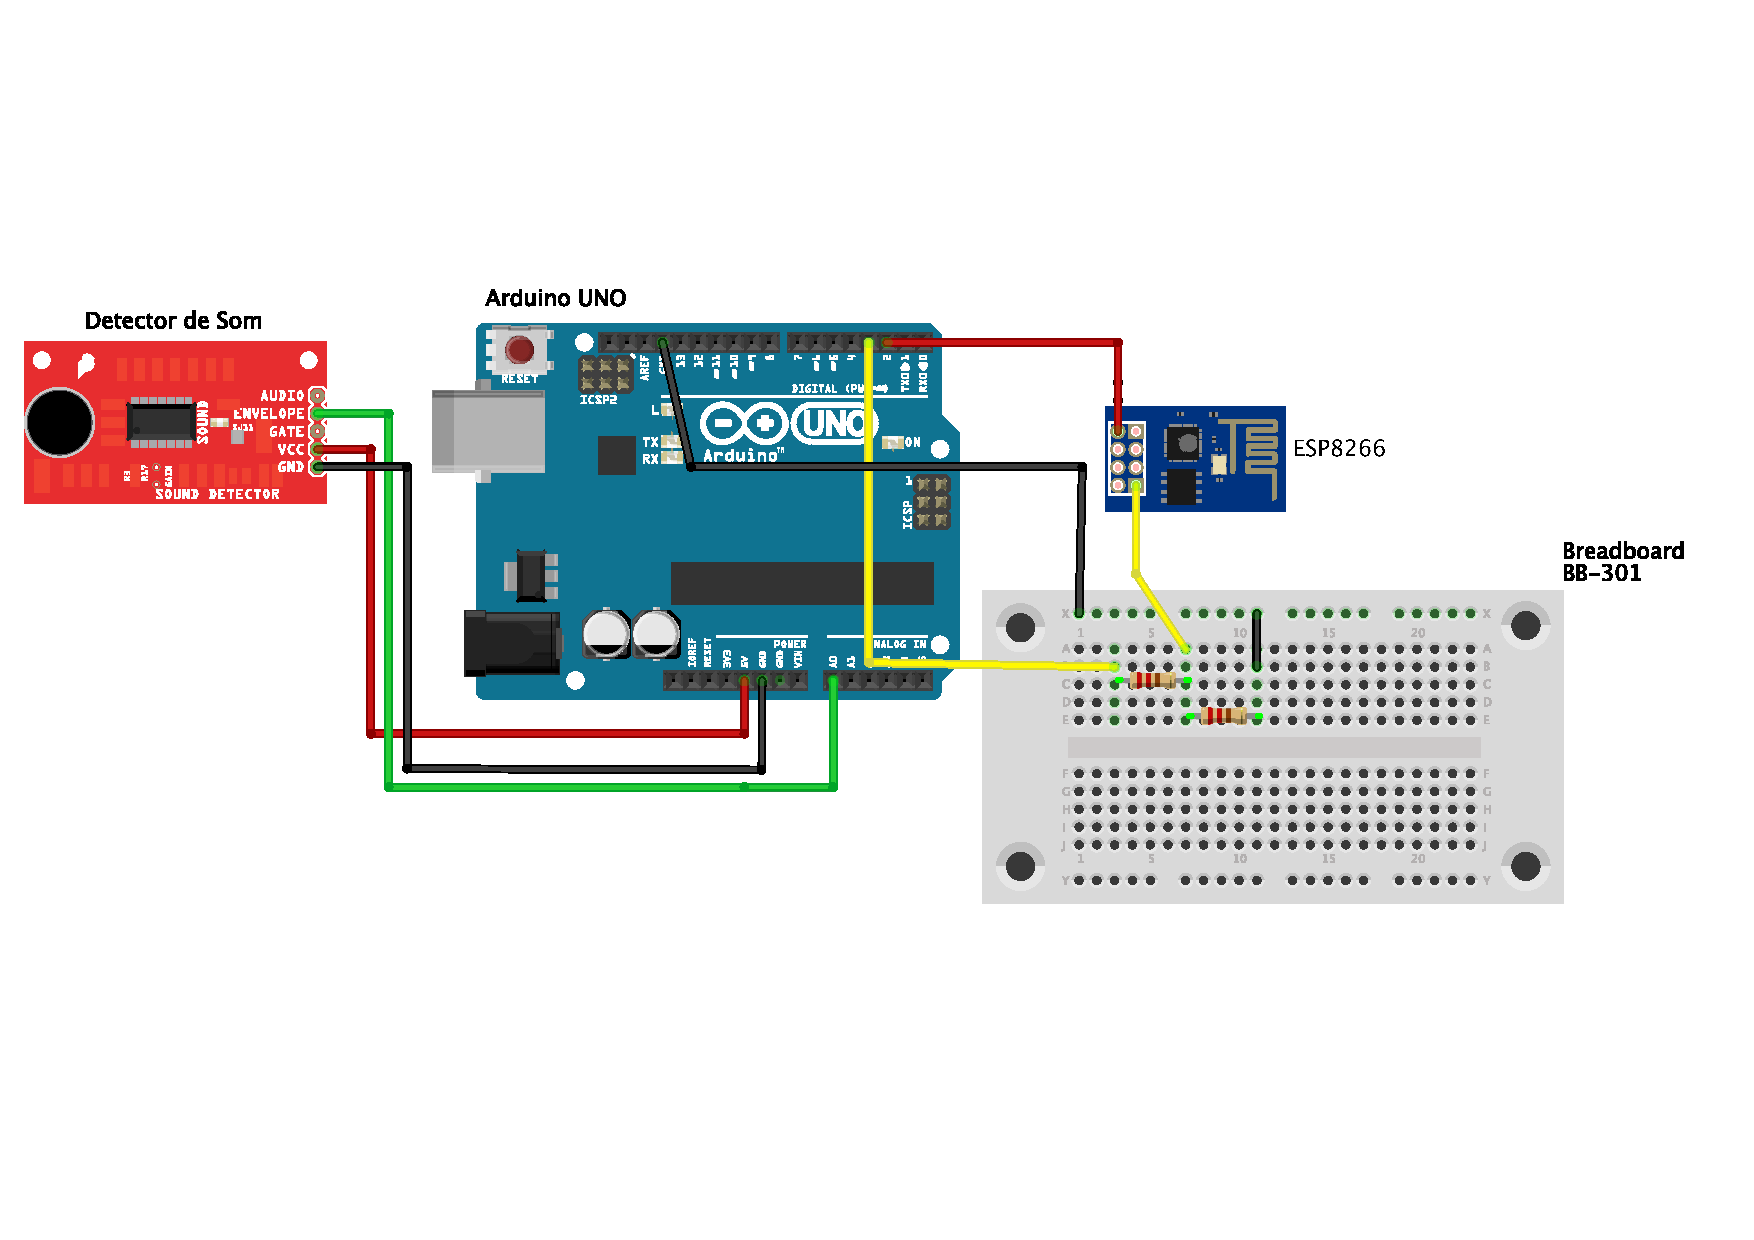
\includegraphics[scale=0.48]{images/circ-2.pdf}
  \end{center}
  \legend{Fonte: o autor.} %http://www.hobbytronics.co.uk/image/cache/data/rapid/16-2-lcd-backlight-green-2-500x500.jpg
\end{figure}

Um outro detalhe importante é que as portas do ESP8266 funcionam em $3,3V$. Sendo assim, para a conexão do módulo ao \textit{Arduino}, foi utilizado um divisor de tensão (reduzindo o valor de tensão) para conectar a porta \texttt{3} (cuja saída é $5V$) do \textit{Arduino} à porta \textit{RX} do ESP.

Como se pode ver na Figura \ref{circ-2}, as portas \texttt{2} e \texttt{3} foram utilizadas para fazer a comunicação serial entre o \textit{Arduino} e o Módulo (\textit{Arduino} \texttt{2} como $RX$ $\Rightarrow$ $TX$ do Módulo, \textit{Arduino} \texttt{3} como $TX$ $\Rightarrow$ $RX$ do Módulo). Esta configuração já permite fazer criar um programa para rodar no \textit{Arduino} que efetue a leitura de um valor de amplitude sonora com o DDS, e envie para um servidor \textit{web} utilizando o ESP8266.

\subsection{Arduino e LCD}

As portas de \texttt{4} a \texttt{7} do \textit{Arduino} foram conectadas aos pinos de dados do LCD. Já as portas \texttt{8} e \texttt{9} foram conectadas ao LCD para que fosse possível a leitura e escrita de dados.

\begin{figure}[!htb]
  \begin{center}
    \caption{\label{circ-3}Conexão entre \textit{Arduino}, display de LCD e demais componentes.}
    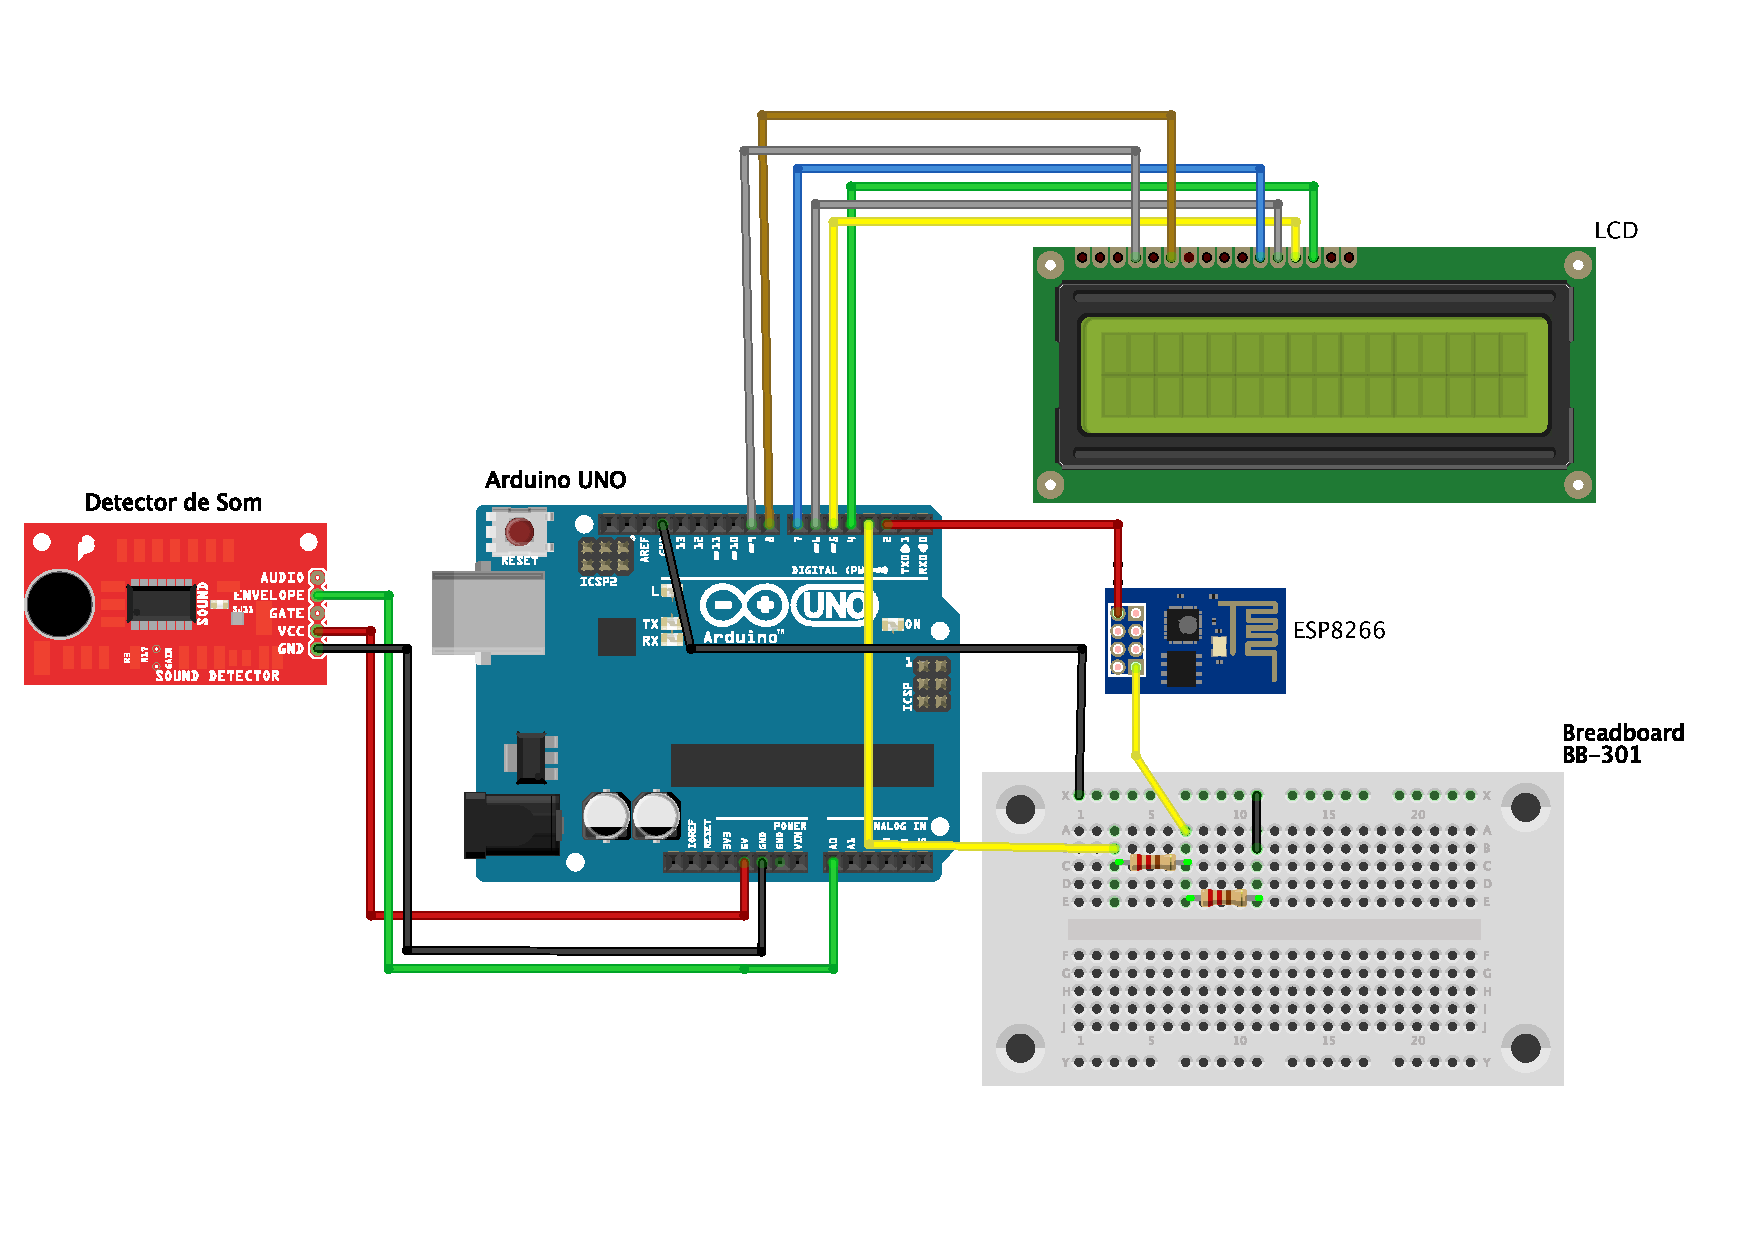
\includegraphics[scale=0.48]{images/circ-3.pdf}
  \end{center}
  \legend{Fonte: o autor.} %http://www.hobbytronics.co.uk/image/cache/data/rapid/16-2-lcd-backlight-green-2-500x500.jpg
\end{figure}

Os demais ajustes, incluindo \textit{backlight} e contraste, bem como alimentação e terra, pode ser vistos no \textit{hardware} final. O brilho do \textit{backlight} foi ajustado utilizando um \textit{trimpot} de $10k\Omega$, e o contraste, um resistor de $1k\Omega$.

\subsection{Arduino e LEDs}

A última parte do projeto do \textit{hardware}, como mencionado previamente, utiliza três LEDs nas cores verde, amarela e vermelha, para indicar a amplitude do som medido. 

\begin{figure}[!htb]
  \begin{center}
    \caption{\label{circ-4}Ilustração do projeto de \textit{hardware} com todos os componentes.}
    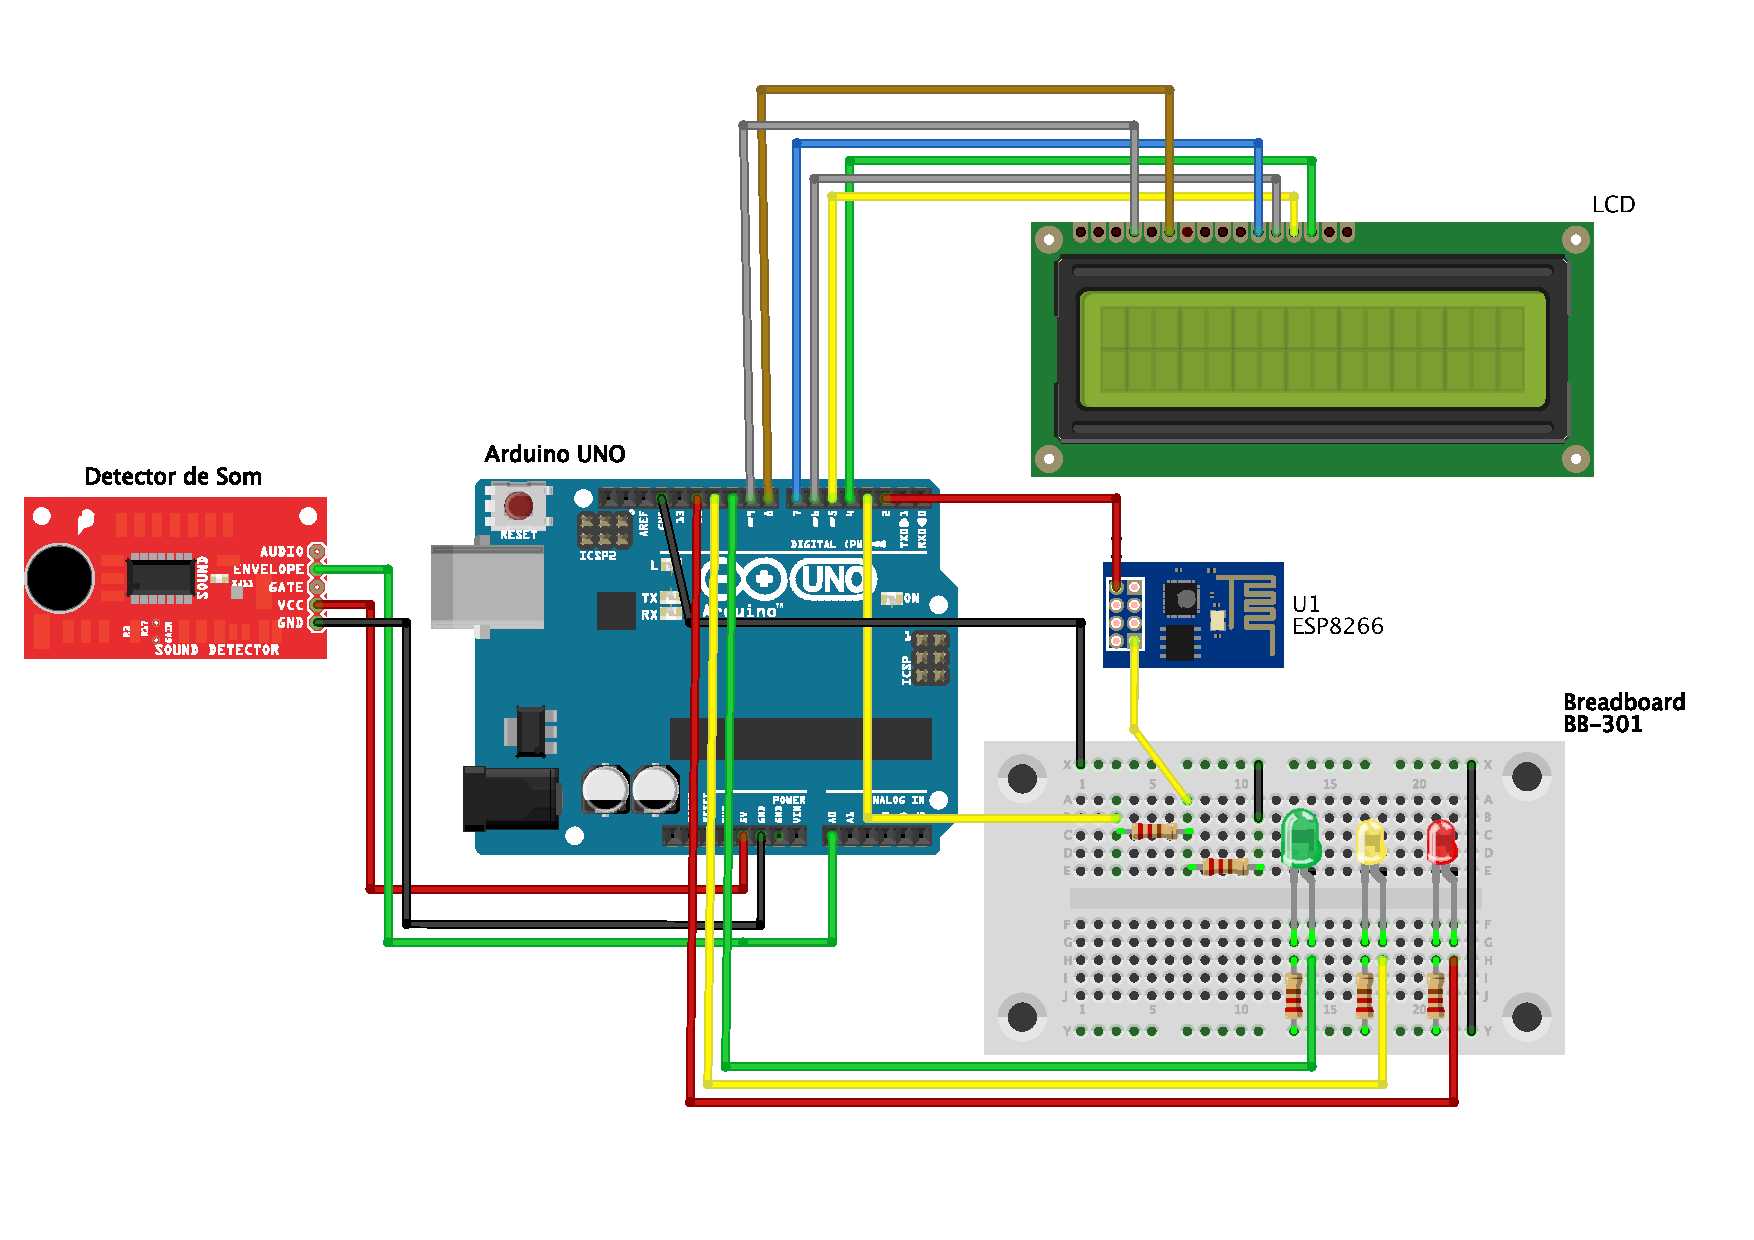
\includegraphics[scale=0.48]{images/circ-4.pdf}
  \end{center}
  \legend{Fonte: o autor.} %http://www.hobbytronics.co.uk/image/cache/data/rapid/16-2-lcd-backlight-green-2-500x500.jpg
\end{figure}

Para isto, foram utilizadas as portas \texttt{10}, \texttt{11} e \texttt{12} do \textit{Arduino} para acender o LED que corresponde a amplitude sonora do local (baixa, alta ou moderada). A Figura \ref{circ-4} ilustra o projeto que foi montado na \textit{protoboard}. 

\subsection{Programa do Microcontrolador}

O programa gravado no \textit{Arduino} possui basicamente três partes (funções) que são:

\begin{enumerate}
   \item \texttt{lcdSetup()}: configura inicialmente o LCD para escrever as informações pro usuário;
   \item \texttt{restartESP()}: configura o ESP para operar no modo estação, se conectando a uma rede WiFi;
   \item \texttt{calculateDecibels():} Leitura do valor analógico em \texttt{A0}, cálculos para encontrar o valor em dB e envio de dados para um servidor \textit{web}.
 \end{enumerate}

No programa escrito em Linguagem C, as diretivas de pré-processamento \texttt{WLAN\_SSID} e \texttt{WLAN\_PASS} definem a rede a qual o ESP irá se conectar.

Assim que o \textit{hardware} é ligado, uma das primeiras etapas que são efetuadas após as configurações iniciais do LCD, é a de tentar conectar-se a rede local.

Em seguida, o programa lê o valor vindo do DDS através do pino analógico \texttt{A0} do Arduino, fornece um valor que equivale ao valor de pico do som. 

O projeto final do medidor na \textit{protoboard} pode ser vistos tanto na Figura \ref{medindo}, exibindo os valores medidos em decibéis, quanto na Figura \ref{setado} que acontece na etapa inicial do sistema, assim que é ligado (por isso os LEDs estão apagados).

Este valor é então passado para a função \texttt{calculateDecibels()} que efetua o cálculo de acordo com a equação \ref{eq-dec}, tendo o valor de referência em decibéis sido estabelecido previamente a partir de um aplicativo de decibelímetro em \textit{software} chamado \textit{Decibels} (processo de calibração). 

\begin{figure}[!htb]
    \centering
    \subfloat[\textit{Status} \textbf{Moderado} (64.72 dB).]{{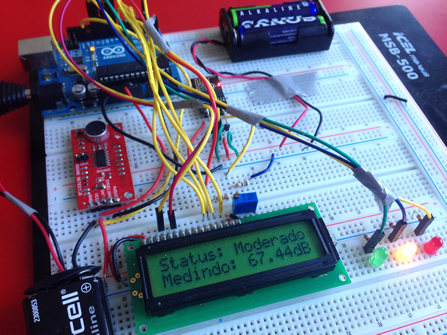
\includegraphics[width=7.2cm]{images/moderado.jpg} }}%
    \qquad
    \subfloat[\textit{Status} \textbf{Alto} (74.64 dB).]{{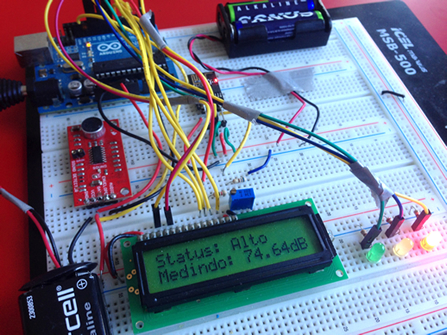
\includegraphics[width=7.2cm]{images/alto.jpg} }}%
    \caption{Projeto do \textit{hardware} montado na \textit{protoboard} medindo o som.}%
    \label{medindo}
\end{figure}

Os valores lidos e menores ou iguais a 55 dB, caracterizam um ambiente \textit{quieto}. Entre 55 dB e 70 dB, um ambiente de som \textit{moderado}, e maiores que 70 dB para um ambiente de som \textit{alto}, valores estabelecidos baseando-se na NBR 10151 da Associação Brasileira de Normas Técnicas (ABNT).

\begin{figure}[!htb]
    \centering
    \subfloat[Sistema conectado ao WiFi no IP \texttt{172.20.10.7}.]{{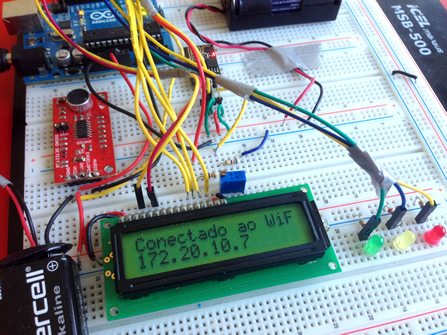
\includegraphics[width=7.2cm]{images/conectado.jpg} }}%
    \qquad
    \subfloat[Módulo ESP configurado em modo estação.]{{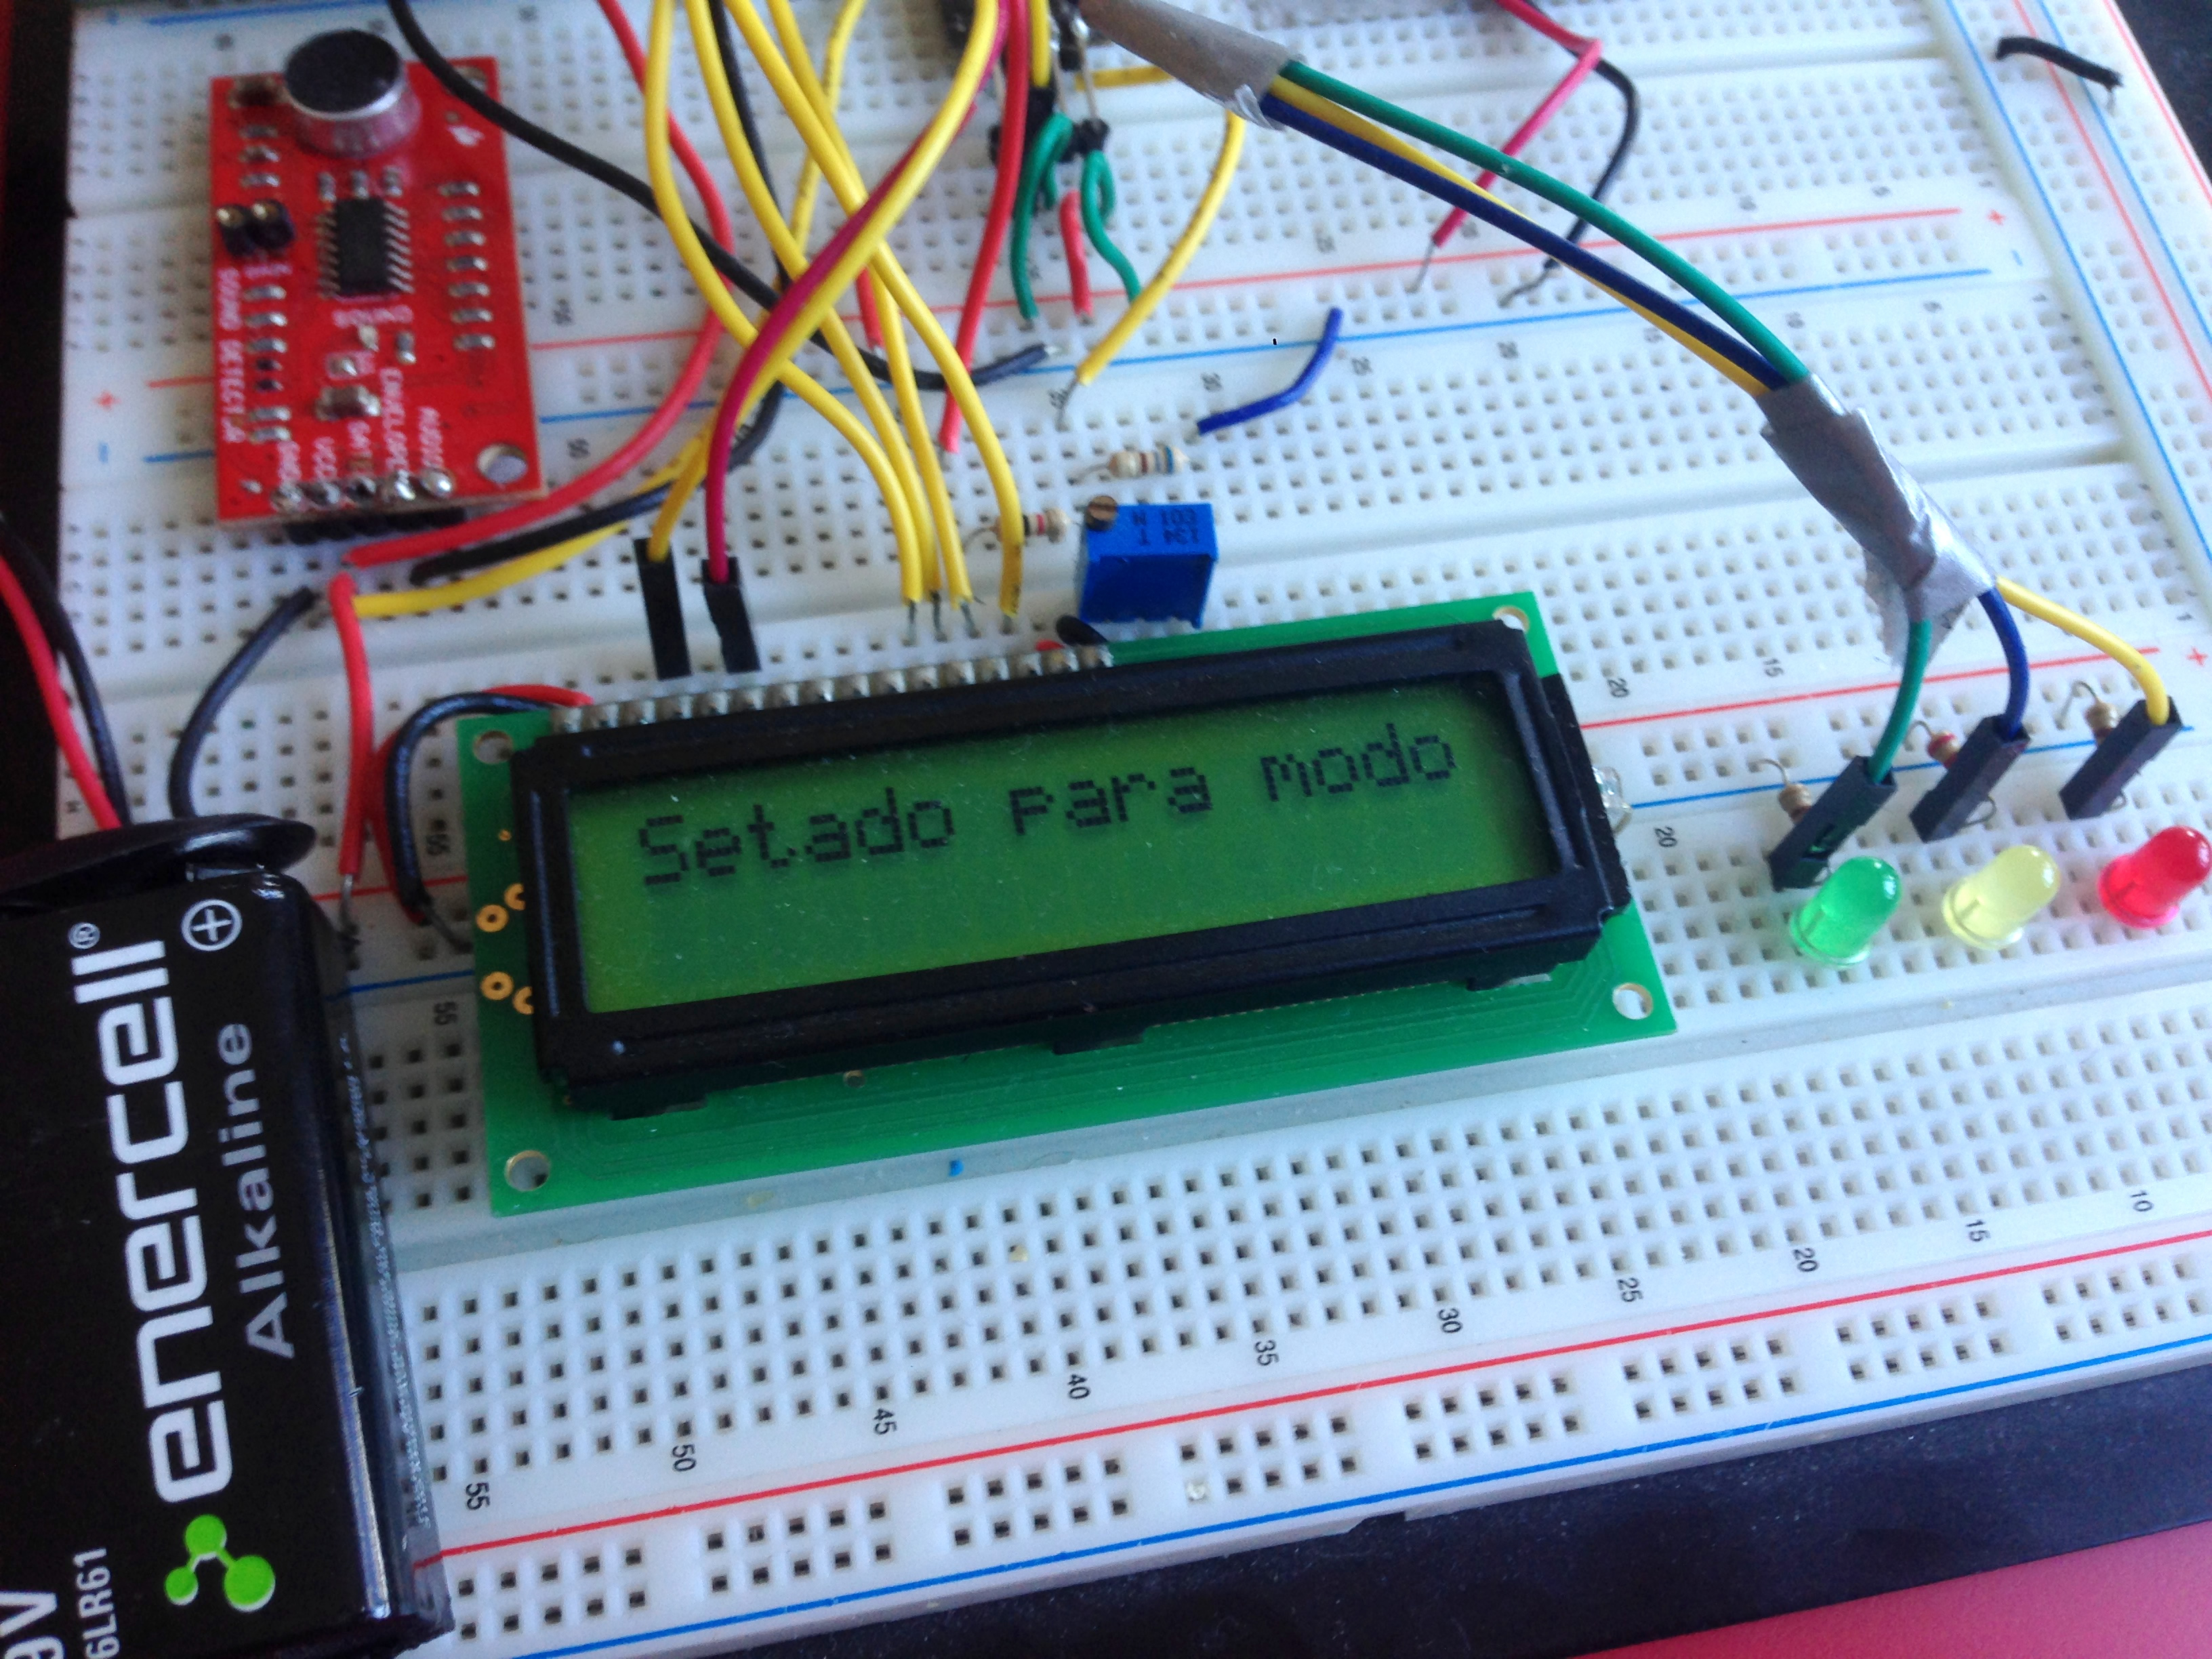
\includegraphics[width=7.2cm]{images/setado.jpg} }}%
    \caption{Projeto do \textit{hardware} montado na \textit{protoboard} antes de medir: conectando-se à rede.}%
    \label{setado}
\end{figure}

O projeto final do medidor na \textit{protoboard} pode ser visto tanto na Figura \ref{medindo}, exibindo os valores medidos em decibéis, quanto na Figura \ref{setado} que exibe a etapa inicial do sistema, momentos após ser ligado (por isso os LEDs estão apagados).

\section{Projeto de \textit{Software}}\label{projeto-soft}

O projeto do \textit{software} de monitoramento dos dados medidos pelo \textit{hardware} desenvolvido na Seção anterior ser uma aplicação \textit{mobile}, levou em consideração o fato de que o Brasil ocupa a sexta posição em número de \textit{smartphones} no mundo.

Embora dispositivos com sistema operacional \textit{Android} ainda ocupem a primeira posição no mercado brasileiro (por fatores como variedade de aparelhos, faixa de preços e assim por diante), até julho deste ano, o sistema operacional iOS da \textit{Apple} estava em terceiro lugar.

Logo, decidiu-se por desenvolver uma aplicação \textit{mobile} para dispositivos iOS, que fosse capaz de localizar os pontos em que os dispositivos de \textit{hardware} estão instalados, e ao mesmo tempo, pudesse exibir os valores medidos em tempo real.

As etapas do processo de desenvolvimento do \textit{software} para dispositivos móveis rodando o sistema operacional iOS, é descrita a seguir juntamente com uma breve explicação das ferramentas utilizadas.

\subsection{Sistema Operacional iOS}

iOS é um sistema operacional da \textit{Apple Inc.} que roda em dispositivos iPhone, iPad e iPod Touch. Além de gerenciar os recursos de \textit{hardware} de tais dispositivos, tal sistema operacional (SO) também provê as tecnologias necessárias para o desenvolvimento de aplicações nativas.

\begin{figure}[!htb]
  \begin{center}
    \caption{\label{iphone}iPhone: exemplo de dispositivo que roda o sistema operacional iOS.}
    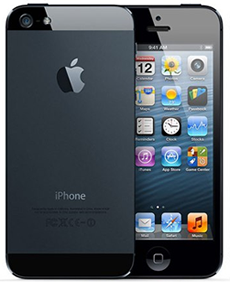
\includegraphics[scale=0.39]{images/iphone.png}
  \end{center}
  \legend{Fonte: extraído de \cite{iphoni}} %http://www.hobbytronics.co.uk/image/cache/data/rapid/16-2-lcd-backlight-green-2-500x500.jpg
\end{figure}

O principal diferencial do iOS em relação aos demais SOs no que diz respeito ao desenvolvimento de aplicações, é a robustez do seu \textit{kit} de desenvolvimento de \textit{software}, \textit{Software Development Kit} (SDK).

O iOS SDK possui uma série completa de ferramentas para desenvolver, instalar, rodar e testar aplicações para dispositivos iOS que são criadas utilizando-se de sua enorme gama de \textit{frameworks} e do poder da linguagem \textit{Objective-C}. 

\subsection{\textit{Objective-C}}

Embora a \textit{Apple} tenha lançado recentemente uma nova linguagem (\textit{Swift}) com o intuito de facilitar a programação e crescer o número de desenvolvedores para seus dispositivos, \textit{Objective-C} desde a primeira versão do sistema operacional, tem sido a linguagem de programação utilizada para este fim. 

Mesmo com o rápido crescimento de \textit{Swift}, a maioria esmagadora de bibliotecas encontra-se implementada em \textit{Objective-C}, sendo assim ainda bastante utilizada no desenvolvimento para iOS. 

\begin{figure}[!htb]
  \begin{center}
    \caption{Exemplo de método em \textit{Objective-C}: muito semelhante a C.}
    \begin{verbatim}
                        - (int)tamanhoDeCaracteres {
                            int numeroDeCaracteres = 10;
                            numeroDeCaracteres += 20;
                            return numeroDeCaracteres;
                        }
    \end{verbatim}
    \legend{Fonte: o autor.}
  \end{center}
\end{figure}
\textit{Objective-C} é definida como uma modificação da linguagem C para prover a utilização de orientação a objetos e \textit{dynamic runtime}, que é a capacidade de definir qual implementação de método chamar, antes de fazê-lo.

Ainda assim, \textit{Objective-C} herda os tipos primitivos, sintaxe e estruturas de controle de fluxo de C.

\subsection{\textit{XCode}}

A principal ferramenta no desenvolvimento de aplicações para iOS é o \textit{XCode}. O \textit{XCode} é um ambiente de desenvolvimento integrado, \textit{Integrated Development Environment} (IDE), utilizado para construir desde a interface que o usuário vai utilizar (botões e telas), até o código que determina o comportamento da aplicação.

% \begin{figure}[!htb]
%   \begin{center}
%     \caption{\label{xcode}\textit{XCode}: IDE de desenvolvimento de aplicações para iOS.}
%     \includegraphics[scale=0.29]{images/xcode7.png}
%   \end{center}
%   \legend{Fonte: extraído de \cite{logo-xcode}} %http://www.hobbytronics.co.uk/image/cache/data/rapid/16-2-lcd-backlight-green-2-500x500.jpg
% \end{figure}

Devido ser uma ferramenta \textit{all-in-one} e de fácil adaptação, o \textit{XCode} é uma das razões que tornam o desenvolvimento de aplicações para \textit{iOS} uma tarefa menos dispendiosa, aumentando a velocidade de programação e facilitando a depuração de código. 

É importante salientar que o \textit{XCode} também pode ser utilizado para criação de aplicações em linguagem C e C++.

\subsection{Servidor \textit{Web}: Plataforma \textit{ThingSpeak}}

Nas primeiras Seções descrevendo o comportamento desejado do sistema, foi estabelecido que os dados lidos pelo \textit{hardware} seriam enviados pela Internet (através do Módulo ESP8266), e acessados via \textit{sofware} pela aplicação móvel.

Deste modo, a plataforma escolhida como servidor \textit{web} para abrigar tais dados foi a \textit{ThingSpeak}, uma plataforma de dados \textit{open-source} da \textit{MathWorks Inc.}, empresa detentora do mundialmente conhecido \textit{software} MATLAB.

% \begin{figure}[!htb]
%   \begin{center}
%     \caption{\label{things}\textit{ThingSpeak}: plataforma \textit{web} e \textit{open-source} para dispositivos embarcados.}
%     \includegraphics[scale=0.37]{images/thingspeak.png}
%   \end{center}
%   \legend{Fonte: extraído de \cite{logo-things}}. %http://www.hobbytronics.co.uk/image/cache/data/rapid/16-2-lcd-backlight-green-2-500x500.jpg
% \end{figure}

O \textit{ThingSpeak} permite que dispositivos embarcados conectados a Internet possam armazenar e visualizar dados de sensores ou atuadores, como \textit{Arduino}, \textit{Raspberry Pi} e assim por diante. O funcionamento do \textit{ThingSpeak} baseia-se no conceito de \textit{canais}, os quais contém atributos de dados como \textit{status}, localização e outros. 

Após a criação de um canal, a plataforma fornece um identificador que pode ser utilizado nas chamadas da sua Interface de Programação de Aplicação, \textit{Application Programming Interface} (API), para escrita e leitura de dados do canal a partir de requisições utilizando o Protocolo de Transferência de Hipertexto, \textit{Hypertext Transfer Protocol} (HTTP). Além do mais, a \textit{ThingSpeak} disponibiliza em sua documentação uma lista de palavras chave para o entendimento de sua API e que serão utilizados na descrição dos resultados do projeto. 

Dentre elas:

\begin{itemize}
  \item \textbf{Canal:} nome do local onde os dados podem ser inseridos ou recuperados, identificado por um identificador numérico. Exemplo: \texttt{57789};
  \item \textbf{Campo:} localização específica (são possíveis até 8) para os dados inseridos no canal. Um campo pode armazenar caracteres alfanuméricos. Exemplo: \texttt{decibeis = 44.50};
  \item \textbf{Localização:} latitude e longitude de onde o dado está sendo enviado;
  \item \textbf{\textit{Feed}}: nome para o conjunto de dados armazenados no canal, como latitude, longitude, campos e outros;
  \item \textbf{Chave de Escrita:} um código de 16 dígitos que permite uma aplicação escrever dados no canal. Exemplo: \texttt{AO4V0RJJ7F022KMJ};
  \item \textbf{Chave de Leitura:} um código de 16 dígitos que permite uma aplicação ler dados do canal.
\end{itemize}

\section{Funcionamento do \textit{Software} de Monitoramento}

Utilizando-se do \textit{framework} de mapas do iOS, o \texttt{MapKit}, foi desenvolvida uma aplicação chamada \textit{Recife SM} (\textit{Recife Sound Monitoring}) capaz de exibir as localizações de pontos da cidade em que o \textit{hardware} acima desenvolvido for instalado.

Supondo que o \textit{hardware} tivesse sido instalado em quatro pontos do Recife Antigo, o usuário seria capaz de verificar informações sobre o barulho naquele local a qualquer momento, a partir do seu dispositivo iOS.  Os locais escolhidos para a inserção no possível mapa de poluição sonora do Recife foram alguns estabelecimentos comerciais e um ponto turístico da cidade, na área da Praça do Marco Zero.

Como se pode ver na Figura \ref{rodando}, a tela inicial mostra os pontos da cidade para que o usuário possa escolher que local vai querer obter informações sobre o som do ambiente naquele momento. 


\begin{figure}[!htb]
  \caption{Telas iniciais do \textit{software} de monitoramento.}
    \centering
    \subfloat[Tela inicial: pontos da cidade no mapa.]{{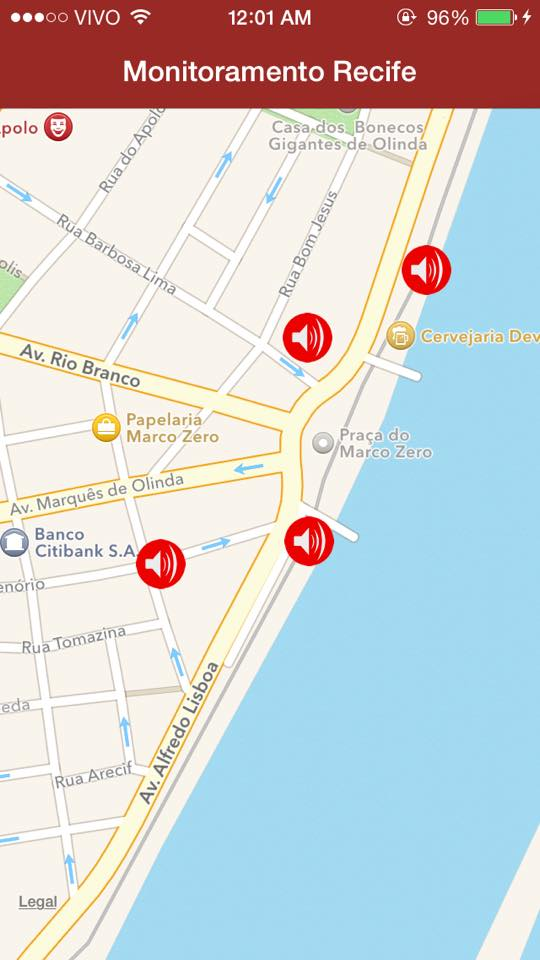
\includegraphics[width=5cm]{images/tela1-mod.jpg}}}%
    \qquad
    \subfloat[Usuário escolhe o local ao tocar no ponto do mapa.]{{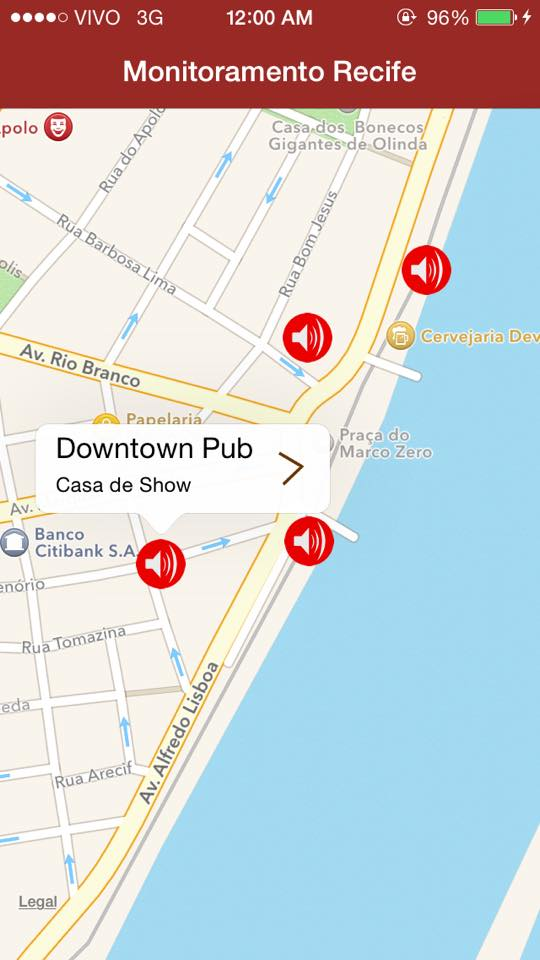
\includegraphics[width=5cm]{images/tela2-mod.jpg}}}%%
    \label{rodando}
\end{figure}

% \begin{figure}[!htb]
%   \begin{center}
%     \caption{\label{tela1}Tela inicial do aplicativo de monitoramento: pontos da cidade no mapa.}
%     \includegraphics[scale=0.2]{images/tela1.jpg}
%   \end{center}
%   \legend{Fonte: o autor.} %http://www.hobbytronics.co.uk/image/cache/data/rapid/16-2-lcd-backlight-green-2-500x500.jpg
% \end{figure}

O usuário então toca nos pontos do mapa e escolhe que local deseja saber detalhes, podendo monitorar o barulho no ambiente de qualquer lugar, com seu \textit{smartphone} e acesso a Internet. É possível ver que o usuário tem a opção de escolher que local ele deseja monitorar. A seta do lado direito indica que é possível saber mais detalhes a respeito daquele local escolhido.

Ao abrir a tela de Detalhes, como visto na Figura \ref{tela3}, o usuário além de visualizar o valor do som do ambiente em decibéis, pode também efetuar uma ligação ou comunicar por e-mail o local que esteja ultrapassando os limites estabelecidos pelos órgãos da cidade. 

\begin{figure}[!htb]
  \begin{center}
    \caption{\label{tela3}Tela de detalhes do local escolhido pelo usuário: dados do medidor.}
    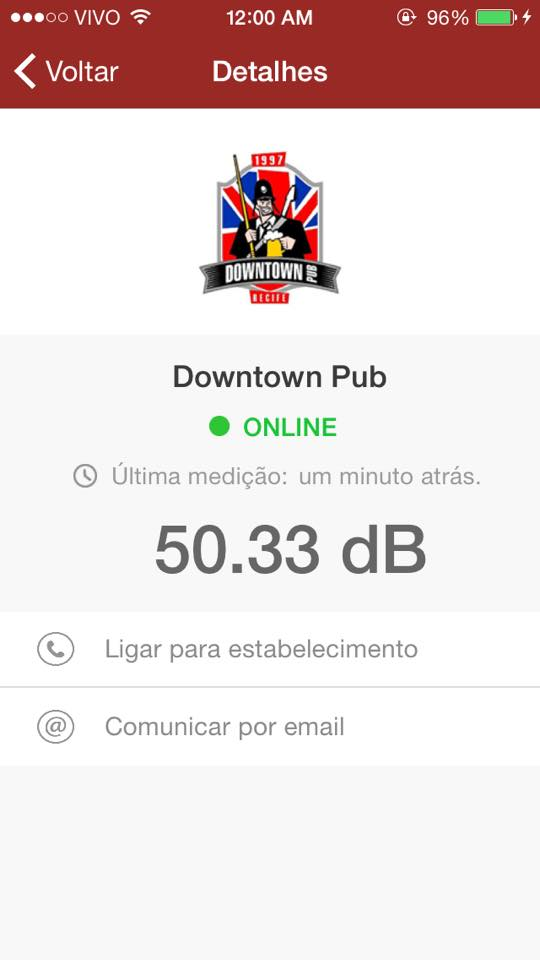
\includegraphics[scale=0.25]{images/tela3-mod.jpg}
  \end{center}
  \legend{Fonte: o autor.} %http://www.hobbytronics.co.uk/image/cache/data/rapid/16-2-lcd-backlight-green-2-500x500.jpg
\end{figure}

\chapter{Resultados e Testes}\label{resultados}

Este capítudo descreve os testes realizados com as ferramentas desenvolvidas tanto em \textit{hardware} quanto em \textit{software}. Na Seção \ref{medicoes}, o medidor foi ligado para efetuar medidas de valores de decibeis e compará-las com um medidor em \textit{software}, calculando-se o erro entre os valores. 

Em seguida, na Seção \ref{things-sec}, foi analisado o comportamento do circuito durante a fase de envio de dados para a plataforma \textit{ThingSpeak}, bem como exibido alguns detalhes do comportamento do programa do \textit{Arduino} nas requisições HTTP. 

Por fim, a Seção \ref{soft} explica os testes realizados no momento da leitura dos dados da plataforma \textit{web}.

\section{Medições do \textit{Hardware}}\label{medicoes}

Logo após o projeto desenvolvido, o sistema foi ligado para algumas medições e comparações. Como não foi possível obter um MNPS profissional para comparação, os valores obtidos foram comparados com os de uma aplicação MNPS em \textit{software}, o aplicativo \textit{Decibels}.

Para um ambiente de uma sala com pessoas conversando próximo aos medidores, obtiveram-se os seguintes valores:

  \begin{table}[!htb]
    \caption{Tabela com valores em dB das medições do \textit{hardware} e do aplicativo \textit{Decibels}. }
    \label{tabela-db}
    \center
    \begin{tabular}{|c|c|}
      \hline
      \rowcolor[gray]{.9}
      \textbf{\textit{Hardware} desenvolvido} & \textbf{Aplicativo \textit{Decibels}}\\
      \hline
      \textsf{66.52} & \textsf{68.13}\\
      \hline
      \textsf{75.22} & \textsf{79.15}\\
      \hline
      \textsf{66.03} & \textsf{68.20}\\
      \hline
      \textsf{65.89} & \textsf{69.17}\\
      \hline
      \textsf{73.69} & \textsf{79.91}\\
      \hline
      \textsf{68.65} & \textsf{68.23}\\
      \hline
      \textsf{66.52} & \textsf{70.12}\\
      \hline
      \textsf{66.99} & \textsf{68.79}\\
      \hline
      \textsf{67.12} & \textsf{69.87}\\
      \hline
    \end{tabular}
  \end{table} 

De posse dos valores da Tabela \ref{tabela-db}, é possível calcular um erro médio que relaciona o que foi medido pelo \textit{hardware} e o valor ideal medido pelo aplicativo. Assim, sendo $x_i$ o valor medido pelo \textit{hardware} e $\hat{x}_{i}$ o valor ideal obtido do aplicativo, o erro médio absoluto $e$ é dado por: 
 \begin{align}
  e = \frac{\sum_{i=1}^{N} |x_{i}-\hat{x}_{i}|}{N} = \frac{24.94}{10} \Rightarrow \boxed{e = 2.494} \ (dB)
 \end{align}

O erro absoluto $e$ de $2.494$ mostra que os valores medidos pelo \textit{hardware} estão bem próximos de um MNPS confiável, mesmo que em \textit{software}. 

Também, a partir dos dados exibidos na Tabela \ref{tabela-db}, foi plotado o Gráfico \ref{graf} que ilustra a proximidade dos valores medidos. 

\begin{figure}[!htb]
  \caption{Gráfico de medições do \textit{hardware} $\times$ aplicativo \textit{Decibels} (\textit{software}).}\label{graf}
  \begin{center}
    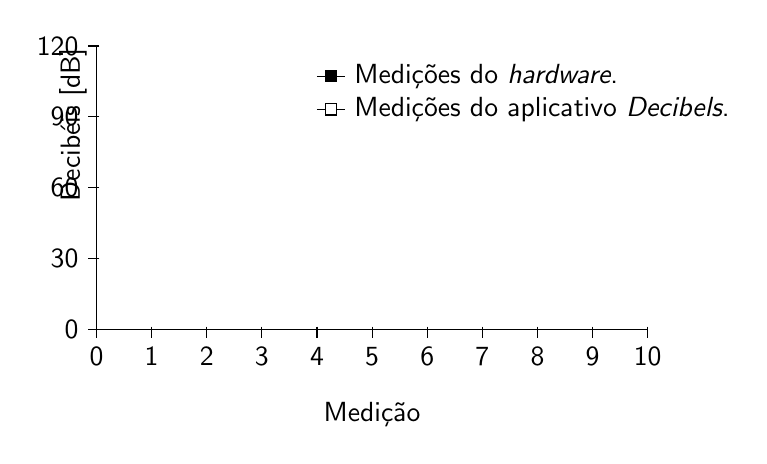
\begin{tikzpicture}[y=.03cm, x=.7cm,font=\sffamily]
      %axis
      \draw (0,0) -- coordinate (x axis mid) (10,0);
          \draw (0,0) -- coordinate (y axis mid) (0,120);
          %ticks
          \foreach \x in {0,...,10}
            \draw (\x,1pt) -- (\x,-3pt)
          node[anchor=north] {\x};
          \foreach \y in {0,30,...,120}
            \draw (1pt,\y) -- (-3pt,\y) 
              node[anchor=east] {\y}; 
      %labels      
      \node[below=0.8cm] at (x axis mid) {Medição};
      \node[rotate=90, above=0.8cm] at (y axis mid) {Decibéis [dB]};

      \draw plot[mark=square*]
        file {data/div_ciu_oscar_extrapolated.data};

      \draw plot[mark=square*, mark options={fill=white}]
        file {data/decibels.data}; 
        
      %legend
      \begin{scope}[shift={(4,65)}] 
      \draw[yshift=3\baselineskip] (0,0) -- 
        plot[mark=square*, mark options={fill=black}] (0.25,0) -- (0.5,0)
        node[right]{Medições do \textit{hardware}.};
      \draw[yshift=2\baselineskip] (0,0) -- 
        plot[mark=square*, mark options={fill=white}] (0.25,0) -- (0.5,0)
        node[right]{Medições do aplicativo \textit{Decibels}.};
      \end{scope}
    \end{tikzpicture}
  \end{center}
  \legend{Fonte: o autor.}
\end{figure}

O ideal seria o uso de um MNPS profissional para fazer outras comparaçãos e definir a precisão do projeto desenvolvido a partir de outros testes e ambientes. No entanto, os resultados para o medidor foram bastante satisfatórios e a precisão condizente com o esperado.

% \subsection{Gráfico do campo Decibéis}
% Mostrar tabela de valores em dB durante certo tempo funcionando.. Gráfico comparando valores aplicativ. decib. vs meu medidor, 
% comentar q está funcionando conforme projetado, com um erro de x, deixar claro que a proposta nao é ser um medidor extremamente preciso ou profissional a priori, mas de baixo custo e fácil uso etc e pra este proposito está oK

% Comentar sobre o motiv da alimentacao isolada do esp (duas AA de 1,5v) e consumo de ate 300mA, drena mta bateria rapido / Dizer que o led azul dele acende no momento de envio do dado

\section{Processo de Atualização e Leitura na \textit{ThingSpeak}}\label{things-sec}

\subsection{Escrita dos valores via \textit{hardware}}

Como explicitado anteriormente, existem duas chaves de acesso (leitura e escrita) a um canal do \textit{ThingSpeak}, sendo a de escrita utilizada para atualização do canal. 

Após o desenvolvimento do \textit{hardware} efetuando a leitura dos valores em decibéis e exibindo-os no LCD, um dos fatores para demonstrar o correto funcionamento do projeto seria o envio de dados para o servidor da \textit{ThingSpeak}. Sendo assim, foi criado um canal na plataforma para o qual a API do \textit{ThingSpeak} gerou duas chaves distintas de escrita e leitura. Também foi adicionado ao canal o campo \texttt{field1:Decibeis} para receber o valor medido pelo \textit{hardware}.

Para a realização dos testes, foi criado um canal de exemplo (no modo de acesso privado) de um hipotético estabelecimento comercial sendo monitorado.\footnote{a \textit{logo} do estabelecimento é exibida apenas a nível de ilustração e demonstração de funcionamento do sistema} A cada 1 minuto, o programa rodando no \textit{Arduino} realizou a chamada \texttt{void sendToThingSpeak(float valueInDecibels)} que recebia o valor final calculado em decibéis, e criava uma conexão TCP com o IP da \textit{ThingSpeak} (\texttt{184.106.153.149}). 

Sendo \texttt{IGPEC0UJCH5I6IAY} a chave de escrita gerada pela plataforma, montou-se a chamada \texttt{GET} incubida de atualizar o canal.

Logo, a chamada montada no programa:

\begin{verbatim}
                    GET /update?key=IGPEC0UJCH5I6IAY&field1=%s
\end{verbatim}

(sendo \texttt{s} o valor em decibéis armazenado na variável \texttt{valueInDecibels}) fez a escrita no canal de acordo com o esperado. Na Figura \ref{cinq} pode-se ver diretamente no LCD o sistema efetuando uma leitura de 48.58 dB momentos antes de iniciar o processo de envio para a \textit{ThingsSpeak} descrito acima:

\begin{figure}[!htb]
  \begin{center}
    \caption{\label{cinq}Sistema medindo 51.08 dB momentos antes de enviar.}
    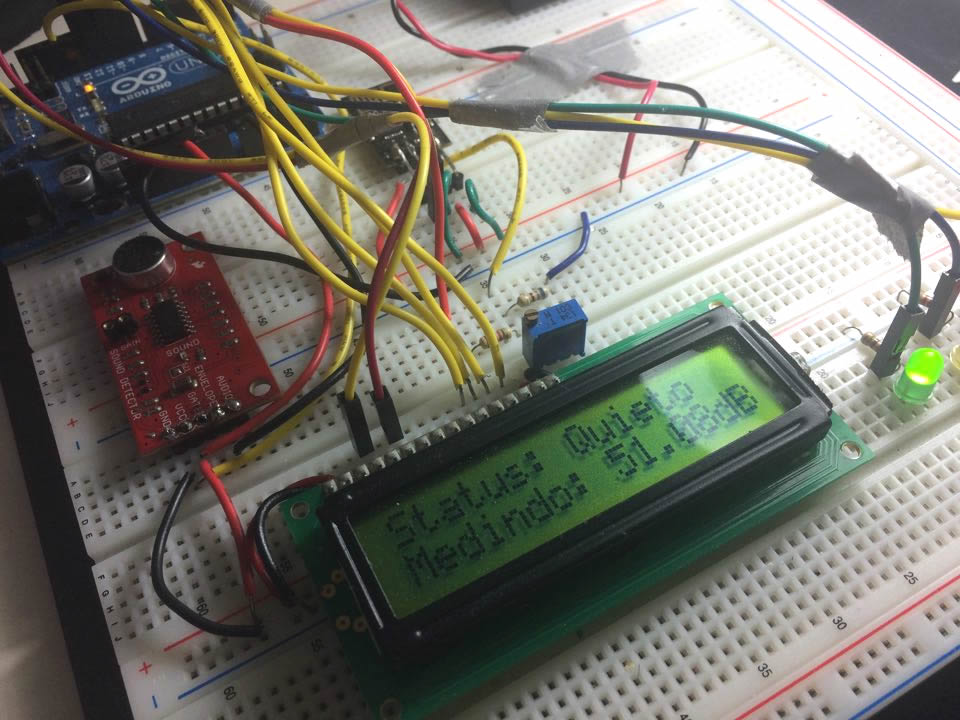
\includegraphics[scale=0.19]{images/cinq.jpg}
  \end{center}
  \legend{Fonte: o autor.} %http://www.hobbytronics.co.uk/image/cache/data/rapid/16-2-lcd-backlight-green-2-500x500.jpg
\end{figure} 

Para verificar a autonomia e estabilizade do sistema, o mesmo foi deixado ligado com alimentação de uma bateria de 9V e duas pilhas AA de 1,5V cada especialmente para o módulo ESP, medindo o ambiente de uma sala com pessoas conversando por pouco mais de uma hora e quarenta minutos. Abaixo vê-se o gráfico Tempo $\times$ Decibéis gerado com os valores obtidos.

\begin{figure}[!htb]
  \begin{center}
    \caption{\label{erre}Gráfico com valores medidos pelo sistema em decibéis durante 100 minutos.}
    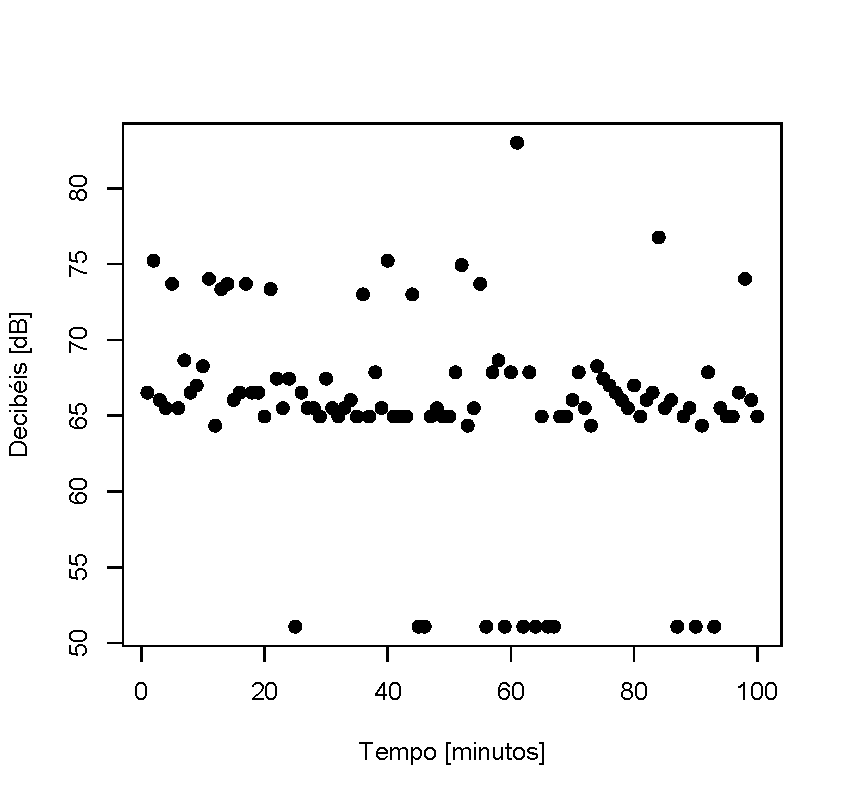
\includegraphics[scale=0.56]{images/Rplot.pdf}
  \end{center}
  \legend{Fonte: o autor.} %http://www.hobbytronics.co.uk/image/cache/data/rapid/16-2-lcd-backlight-green-2-500x500.jpg
\end{figure}

O Gráfico \ref{erre} mostra que dos 100 valores de decibéis medidos, a maior parte se encontra entre 65 e 70 decibéis, o que resulta em um ambiente com \textit{status} de moderado, o que era esperado como comportamento ideal (para a situação testada) no processo de medição pelo sistema. 

\subsection{Leitura dos valores via \textit{software}}\label{soft}

Para lefetuar a leitura dos valores escritos na plataforma a partir da chave de leitura (\texttt{AO4V0RJJ7F022KMJ}), a aplicação rodando no iOS efetuou uma requisição a partir da URL \small{\texttt{http://api.thingspeak.com/channels/53759/feed/last.json?key=AO4V0RJJ7F022KMJ}}, pois a API fornece essa chamada para acessar apenas o último dado enviado ao canal.

Como exibido na subseção anterior, o valor de 51.08 dB que o medidor apresentava no LCD foi enviado a plataforma e assim, tornou-se acessível pelo aplicativo. 

A Figura \ref{cinqui} exibe o usuário efetuando a leitura do valor em decibéis enviado pelo \textit{hardware} através de conexão WiFi com a rede local:

\begin{figure}[!htb]
  \begin{center}
    \caption{\label{cinqui}\textit{Software} (iOS \textit{app}) efetuando a mesma leitura de 51.08 dB.}
    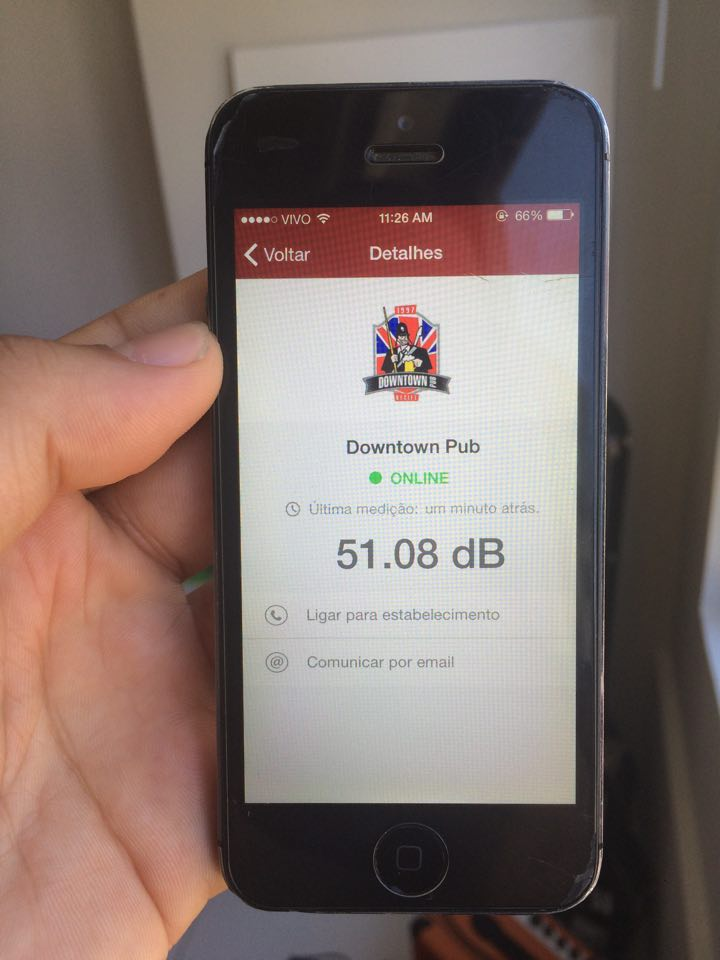
\includegraphics[scale=0.18]{images/cinq-real.jpg}
  \end{center}
  \legend{Fonte: o autor.} %http://www.hobbytronics.co.uk/image/cache/data/rapid/16-2-lcd-backlight-green-2-500x500.jpg
\end{figure}

As requisições HTTP feitas ao \textit{ThingSpeak} retornaram os dados em um formato conhecido por \textit{JavaScript Object Notation} (JSON), o qual contém o identificador da entrada, data de atualização e o valor do campo. 

O \textit{software} então recebe este JSON, e extrai a data de atualização e o valor que corresponde ao medido em decibéis. Para os testes, o retorno da chamada ao serviço foi do tipo:

\begin{verbatim}
    {"created_at":"2015-12-02T05:08:20Z","entry_id":397,"field1":"51.08"}
\end{verbatim}

Este retorno é relativo ao teste executado acima (sistema medindo 51.08 dB), o que possilitou a exibição correta do valor na tela de Detalhes da aplicação. A cada nova chamada os dados de data, identificador e campo eram atualizados. 


% explicar que eh feita uma chamada http especifica pro canal do thingspeak pra pegar somente o ultimo valor enviado, depois o json parser pra exibir o dado e dizer que está func

% Mostrar que o codigo foi compil num iPhone rodando iOS de verdade etc

% \begin{figure}[!htb]
%     \centering
%     \subfloat[Tela inicial do \textit{app}.]{{\includegraphics[width=4cm]{images/mapa.png} }}%
%     \qquad
%     \subfloat[Usuário escolhe local.]{{\includegraphics[width=4cm]{images/mapa2.png} }}%
%     \qquad
%     \subfloat[Aplicação exibe detalhes.]{{\includegraphics[width=4cm]{images/mapa3.png} }}%
%     \caption{\textit{Software} de monitoramento rodando no iOS: iPhone 5.}%
%     \label{rodando}
% \end{figure}

\chapter{Conclusões e Trabalhos Futuros}\label{conclusao}

Neste trabalho foi descrito o processo de desenvolvimento de um sistema de detecção de intensidade sonora, envolvendo a criação de um projeto em \textit{hardware} e \textit{software} capaz de medir um valor em decibéis e enviá-lo para um servidor \textit{web}, automatizando o processo de medição de som.

Durante a realização de testes, percebeu-se que o comportamento do sistema se deu como esperado. Na parte do \textit{hardware}, a fase de detecção e leitura do valor em decibéis, exibição do dado no LCD, LEDs de \textit{status} e envio de dados para o servidor \textit{web} a partir de uma conexão à rede local, foram etapas pré-estabelecidas na fase de projeto e que quando testadas, comportaram-se de maneira adequada.

Também na fase de leitura dos valores pela aplicação em \textit{software} rodando no iPhone, desde a fase de compilação da aplicação no iOS, passando pela montagem da requisição HTTP, recebimento do objeto vindo da \textit{ThingSpeak}, interpretação e exibição de dados para o usuário, também são parte objetivos estabelecidos e atingidos corretamente.

Um dos fatores de melhoramento seria a utilização de um MNPS profissional, que geraria valores mais confiáveis e colocaria a precisão do sistema à prova. Além do mais, um fator que também pode ser testado para atestar a confiabilidade do sistema é o uso contínuo por um longo período de tempo, que trata-se de um cenário mais realista para este tipo de projeto.

A transição do sistema para uma placa de circuito impresso trata-se de um projeto futuro, integrando todos os componentes em um único circuito capaz de ser colocado em um recipiente e instalado em locais desejados como um dispositivo eletrônico comum, eliminando a delicadeza e propensão a erros de ter o circuito montado numa placa de prototipação. 

O desenvolvimento do \textit{software} para outros sistemas operacionais expressivos do mercado seria de grande valia, uma vez que seria capaz de alcançar todas as plataformas \textit{mobile} e aumentaria a popularidade da aplicação, ajudando cidadãos comuns a verificar a qualquer momento a intensidade dos sons emitidos por certos locais da cidade.

A possibilidade do sistema de monitorar o som em decibéis, sendo seu custo total de implementação muito mais baixo que o de um MNPS, e disponibilização deste dado para acesso através de uma aplicação em \textit{software}, torna-o uma ferramenta bastante útil no combate a poluição sonora nos grandes centros urbanos. 

Por fim, implementando-se a opção de comunicar o local dos possíveis danos à saúde causados pelo excesso de barulho (através de e-mail ou ligação) no momento em que tal excesso é verificado, o projeto ganha o potencial de trazer mudança no comportamento das pessoas, induzindo-as a controlar suas emissões de ruídos, contribuindo para um melhor convívio e qualidade de vida. 

% ----------------------------------------------------------
% ELEMENTOS PÓS-TEXTUAIS
% ----------------------------------------------------------
\postextual
% ----------------------------------------------------------

% ----------------------------------------------------------
% Referências bibliográficas
% ----------------------------------------------------------
\bibliography{bib/abntex2-modelo-references}
\bibliographystyle{abntex2-num}
% ----------------------------------------------------------
% Glossário
% ----------------------------------------------------------
%
% Consulte o manual da classe abntex2 para orientações sobre o glossário.
%
%\glossary

% ----------------------------------------------------------
% Apêndices
% ----------------------------------------------------------

% ---
% Inicia os apêndices
% ---
% \begin{apendicesenv}

% % Imprime uma página indicando o início dos apêndices
% %\partapendices

% % ----------------------------------------------------------
% \chapter{Quisque libero justo}
% % ----------------------------------------------------------

% \lipsum[50]

% % ---


% % ----------------------------------------------------------
% % Anexos
% % ----------------------------------------------------------

% % ---
% % Inicia os anexos
% % ---
% \begin{anexosenv}

% % Imprime uma página indicando o início dos anexos
% %\partanexos

% % ---
% \chapter{Morbi ultrices rutrum lorem.}
% % ---
% \lipsum[30]

% % % ---
% % \chapter{Cras non urna sed feugiat cum sociis natoque penatibus et magnis dis
% % parturient montes nascetur ridiculus mus}
% % % ---

% % \lipsum[31]

% % % ---
% % \chapter{Fusce facilisis lacinia dui}
% % % ---

% % \lipsum[32]

% \end{anexosenv}

%---------------------------------------------------------------------
% INDICE REMISSIVO
%---------------------------------------------------------------------
\phantompart
\printindex
%---------------------------------------------------------------------

\end{document}
